% CVPR 2023 Paper Template
% based on the CVPR template provided by Ming-Ming Cheng (https://github.com/MCG-NKU/CVPR_Template)
% modified and extended by Stefan Roth (stefan.roth@NOSPAMtu-darmstadt.de)

\documentclass[10pt,twocolumn,letterpaper]{article}

\usepackage[pagenumbers]{cvpr} % To force page numbers, e.g. for an arXiv version

% Include other packages here, before hyperref.
\usepackage{graphicx}
\usepackage{amsmath}
\usepackage{amssymb}
\usepackage{booktabs}

\usepackage{caption}
% \usepackage{subcaption}
\usepackage{array}
\usepackage{multirow}
\usepackage{threeparttable}
\usepackage[dvipsnames]{xcolor}

\newcommand*\rot{\rotatebox{90}}

\usepackage[pagebackref,breaklinks,colorlinks]{hyperref}


% Support for easy cross-referencing
\usepackage[capitalize]{cleveref}
\crefname{section}{Sec.}{Secs.}
\Crefname{section}{Section}{Sections}
\Crefname{table}{Table}{Tables}
\crefname{table}{Tab.}{Tabs.}


\def\cvprPaperID{xxxx} % *** Enter the CVPR Paper ID here
\def\confName{CVPR}
\def\confYear{2023}

\def\ourapproach{SiNC }

\begin{document}

\title{Non-Contrastive Unsupervised Learning of Physiological Signals from Video}

\author{Jeremy Speth, Nathan Vance, Patrick Flynn, Adam Czajka\\
University of Notre Dame\\
{\tt\small \{jspeth,nvance1,flynn,aczajka\}@nd.edu}
}
\maketitle

Answering first-order logical (FOL) queries over knowledge graphs (KG) remains a challenging task mainly due to KG incompleteness. 
Query embedding approaches this problem by computing the low-dimensional vector representations of entities, relations, and logical queries. 
KGs exhibit relational patterns such as symmetry and composition and modeling the patterns can further enhance the performance of query embedding models.
However, the role of such patterns in answering FOL queries by query embedding models has not been yet studied in the literature.
In this paper, we fill in this research gap and empower FOL queries reasoning with pattern inference by introducing an inductive bias that allows for learning relation patterns. 
To this end, we develop a novel query embedding method, RoConE, that defines query regions as geometric cones and algebraic query operators by rotations in complex space. RoConE combines the advantages of Cone as a well-specified geometric representation for query embedding, and also the rotation operator as a powerful algebraic operation for pattern inference. 
%Therefore, RoConE enables inferring patterns during the multi-hop reasoning process.
Our experimental results on several benchmark datasets confirm the advantage of relational patterns for enhancing logical query answering task.
\section{Introduction}
Deep learning~\cite{dl} has been highly successful in computer vision~\cite{sg1,od1,app-detection,zhou2024diffdet4sar,li2024predicting,yang2024saratr,LiSARATRX25}, largely due to the availability of large-scale labeled datasets. However, in many practical scenarios, obtaining such large amounts of labeled data is difficult or costly. To address this challenge, Few-shot learning (FSL) aims to enable models to learn new tasks with only a limited number of labeled samples. Consequently, this problem has garnered significant attention in both academia and industry due to its broad real-world applications. While humans can easily distinguish between objects after seeing only a few examples, machines struggle to achieve similar efficiency. In domains such as natural scene images, large datasets are readily available, but FSL is crucial in scenarios where collecting large amounts of data is difficult. Since the problem was first introduced in 2006~\cite{fsl-1}, numerous methods have been proposed to tackle the challenges of FSL~\cite{fslsurvey,fslsurvey22,fslsurvey20,fsl18,fslsurvey1}.

With the development of FSL, challenges such as limited training data, domain variations, and task modifications have led to the emergence of various FSL variants, including semi-supervised FSL~\cite{semifsl}, unsupervised FSL~\cite{ufsl1,ufsl2}, zero-shot learning (ZSL)\cite{zsl1}, and cross-domain FSL (CDFSL)~\cite{feature-wise,bscd-fsl}, among others. These variants represent distinctive cases of FSL in terms of sample availability and domain learning. This paper focuses specifically on CDFSL variants. The traditional FSL problem assumes that both prior knowledge and target tasks come from the same domain, which is often restrictive in real-world applications. CDFSL addresses this issue by overcoming the domain gap between auxiliary data (which provides prior knowledge) and the target data in FSL tasks, as show in Figure~\ref{int}. For instance, in art image recognition tasks involving scribble, cartoon, or sketch images, FSL could theoretically leverage prior knowledge from related domains like cartoons and sketches. However, such data is often scarce due to copyright restrictions and the high cost of collection. As a result, researchers have turned to data-rich domains, such as natural scene images, to address the challenges of few-shot image recognition in the field of art.
However, the significant domain gap between these domains often leads to performance degradation in FSL. CDFSL faces challenges from both transfer learning and FSL, including domain gaps, class shifts, and the scarcity of labeled samples in the target domain, making it a more complex task. Since its formal introduction in 2020~\cite{feature-wise}, CDFSL has garnered widespread attention, with numerous methods published in top venues~\cite{bscd-fsl,st,dynamic,hybrid_1,feature_reweight_6}. Figure~\ref{imaging} presents the milestones of CDFSL technologies from 2019 to the present, showcasing representative CDFSL methods and related benchmarks.
\begin{figure}%[b]
	\centering
  \vspace{-0.3cm}
 	\includegraphics[width=0.9\linewidth]{CDFSLProblem-10.pdf}
  \vspace{-0.3cm}
	\caption{\textcolor{black}{The difference of few-shot learning and cross-domain few-shot learning.}}
 \vspace{-0.4cm}
	\label{int}
\end{figure}


So far, several surveys have provided comprehensive overviews and future directions for FSL~\cite{fsl18,fslsurvey,fslsurvey1,fslsurvey20,fslsurvey22}. For example,\cite{fsl18} categorizes FSL into experiential and conceptual learning, while\cite{fslsurvey} focuses on empirical risk minimization and defines FSL by experience, task, and performance, introducing CDFSL as a branch of FSL. Both~\cite{fslsurvey1} and~\cite{fslsurvey20} highlight CDFSL as a variant of FSL, discussing meta-learning approaches and benchmarks. Lastly,~\cite{fslsurvey22} offers a taxonomy based on prior knowledge and emphasizes that current methods have yet to fully tackle cross-domain challenges. Collectively, these works point to cross-domain learning as a promising area for future FSL research. Currently, there are two elementary surveys on CDFSL~\cite{wang2023survey,deng2023survey}. \cite{wang2023survey} classifies methods into benchmark, single source, and multiple source categories, while~\cite{deng2023survey} categorizes algorithms into data augmentation and feature alignment paradigms. In contrast, to stimulate future research and help newcomers better understand this challenging problem, this paper offers the first classification grounded in theoretical analysis and provides a comprehensive review, offering deeper insights into the core principles of CDFSL. Firstly, this paper compiles and analyzes a broad range of literature on the topic. An analysis of the reference index reveals that even before the formal introduction of CDFSL, some works had already tried to solve cross-domain issues within the FSL framework~\cite{clc, rffl}. Following its formal introduction as a branch of FSL, CDFSL has garnered significant attention. Additionally, we define CDFSL using both machine learning theory~\cite{ml,erm1} and transfer learning principles~\cite{tltheory}. Secondly, our analysis highlights that the unique challenge in CDFSL lies in the unreliable nature of two-stage empirical risk minimization. The details are discussed in Section~\ref{background}. To address these challenges, the paper organizes CDFSL research into four categories: $\mathcal{D}$-Extension, $\mathcal{H}$-Constraint, $\Delta$-Adaptation, and hybrid approaches. We also compile relevant datasets and benchmarks to evaluate the methods, and analyze their performance, as discussed in Sections~\ref{methods} and~\ref{performance}. Finally, we explore future research directions for CDFSL by considering three perspectives, including problem set-ups, applications, and theories, which provide a comprehensive understanding of the field and its potential for future growth. Contributions of this survey can be summarized as follows:

\begin{itemize}
    \item We analyzed existing CDFSL papers and provided a comprehensive survey. We also defined CDFSL formally, connecting it to classic ML~\cite{ml,erm1} and transfer learning theory~\cite{tltheory}. This helps guide future research in the field.
    \item We listed relevant learning problems for CDFSL with examples, clarifying their relation and differences. This helps position CDFSL among various learning problems. We also analyzed unique issues and challenges of CDFSL, helping to explore a scientific taxonomy for CDFSL work.
    \item We conducted an extensive literature review, organizing it into a unified taxonomy based on $\mathcal{D}$-Extension, $\mathcal{H}$-Constraint, $\Delta$-Adaptation, and hybrid approaches. We introduced applicable scenarios for each taxonomy to help discuss its pros and cons. We also presented datasets and benchmarks for CDFSL, summarizing insights from performance results to improve understanding of CDFSL methods.
    \item We proposed promising future directions for CDFSL in problem set-ups, applications, and theories, based on current weaknesses and potential improvements.
\end{itemize}

\begin{figure}
	\centering
  \vspace{-0.3cm}
        \includegraphics[width=\linewidth]{response/crop_fig2.pdf}
 \vspace{-0.5cm}
	\caption{Chronological milestones of CDFSL from 2019 to the present, including representative CDFSL approaches and related benchmarks. Key events include the release of Meta-Dataset~\cite{meta-dataset} and BSCD-FSL~\cite{bscd-fsl} in 2020, the introduction of pioneering works such as~\cite{feature-wise}, and subsequent contributions like~\cite{feature_reweight_1,lscdfsl}. Later works~\cite{st,dynamic,hybrid_1,hybrid_4,hybrid_2} explored new setups, while~\cite{boosting,ata,data_target_1,feature_reweight_5,parameter_weight_2,confess,feature_reweight_9} focused on improving performance. Please see Section~\ref{methods} for details.}
 \vspace{-0.3cm}
	\label{imaging}
\end{figure}

The remainder of this survey is organized as follows: Section \ref{background} provides an overview of CDFSL, including its definition, challenges, and taxonomy. Section \ref{methods} covers approaches to CDFSL in detail, while Section \ref{performance} presents performance results and evaluates methods. Section \ref{future} explores future directions in set-ups, applications, and theories. Finally, Section \ref{conclusion} concludes the survey.
\section{Background} \label{background}
In this section, we introduce key concepts related to CDFSL in Section \ref{key}, followed by formal definitions of supervised learning, FSL, domain adaptation (DA), and CDFSL with examples in Section \ref{definition}. Section \ref{related} discusses the connections and differences between CDFSL and related problems. In Section \ref{unique}, we cover the challenges that make CDFSL difficult. Finally, Section \ref{taxonomy} presents a unified taxonomy based on how existing works address these challenges.

\subsection{\textcolor{black}{Key Concepts}} \label{key}
To formally define the CDFSL problem, we begin by considering two key concepts: \emph{domain} and \emph{task}~\cite{tfsurvey,tf_2020}. These terms are often used inconsistently in the community, but a clear distinction between them helps in studying different transfer learning subproblems. In this paper, we follow the definitions provided by Pan and Yang's surveys\cite{tfsurvey,tf_2020,tfsurvey_2020}.

% that may differ between the source problem and the target problem

% Before giving our formal definition of CDFSL, we first define two key basic concepts of `domain' and `task' ~\cite{tfsurvey,tf_2020} as their specific contents may differ between the source and target problem, inspired by the excellent survey from Pan and Yang~\cite{tfsurvey}.

%\vspace{-0.2cm}
\begin{MyDef}
\label{def:Domain}
\textbf{Domain.} Given a feature space $\mathcal{X}$ and a marginal probability distribution $P(X)$,  where each input instance $\emph{\textbf{x}}\in\mathcal{X}$, a domain $\mathcal{D}=\{\mathcal{X}, P(X)\}$ consists of $\mathcal{X}$ and $P(X)$.
\end{MyDef}

%\vspace{-0.2cm}
In practice, a domain is often observed by several labeled or unlabeled data samples $X=\{\emph{\textbf{x}}\}_{i=1}^{N}$, where $N$ indicates the number of instances. For instance, if our learning task is image classification, and each input image is represented as a feature vector $\textbf{\emph{x}}$, \eg, by a deep convolution neural network (DCNN), then $\mathcal{X}$ is the space underlying the extracted feature vector. In general,  two different domains can differ in the feature space or the marginal distribution.

%Specifically, for an image domain $\mathcal{D}$, the original images \emph{I} are from a feature space $\mathcal{X}_{I}$, and the corresponding marginal probability distribution is $P(I)$. The image domain $\mathcal{D}$ can be expressed as $\mathcal{D}=\{\mathcal{X}_{I}, P(I)\}$. In general, differences in $\mathcal{X}_{I}$ or $P(I)$ can lead to the different domain $\mathcal{D}$. 

%the original images \textit{I} is mapped to a high-dimensional feature space $\mathcal{X}_{I}$. The features $\textbf{\emph{x}}_{I}$ in $\mathcal{X}_{I}$ is a higher-dimensional abstraction of \textit{I}, and the corresponding marginal probability distribution is $P(\textbf{\emph{x}}_{I})$. The image domain $\mathcal{D}$ can be expressed as $\mathcal{D}=\{\mathcal{X}_{I}, P(\textbf{\emph{x}}_{I})\}$. In general, difference in $\mathcal{X}_{I}$ or $P(\textbf{\emph{x}}_{I})$ can lead to the different domain $\mathcal{D}$. 

%\vspace{-0.5cm}
%\textcolor{black}{
%\begin{MyDef}
%\label{def:Domain}
%\textbf{Domain.} Given a feature space $\mathcal{X}$ and a marginal probability distribution \textit{P(X)}, where $\textit{X}=\{x_{1}, x_{2}, ..., x_{n}\} \subseteq \mathcal{X}$\iffalse, $n$ is the number of instances\fi. A domain $\mathcal{D}=\{\mathcal{X}, \textit{P(X)}\}$ consists of $\mathcal{X}$ and $\textit{P(X)}$.
%\end{MyDef}
%}



% Specifically, for an image domain $\mathcal{D}$, the original images \textit{I} is mapped to a high-dimensional feature space $\mathcal{X}_{I}$. The features $\textit{X}_{I}$ in $\mathcal{X}_{I}$ is a higher-dimensional abstraction of \textit{I}, and the corresponding marginal probability distribution is $P(X_{I})$. The image domain $\mathcal{D}$ can be expressed as $\mathcal{D}=\{\mathcal{X}_{I}, P(X_{I})\}$. In general, difference in $\mathcal{X}_{I}$ or $P(X_{I})$ can lead to the different domain $\mathcal{D}$. 


%\vspace{-0.3cm}
\begin{MyDef}
\label{def:Task}
\textbf{Task.}  Given a domain $\mathcal{D} = \{\mathcal{X}, P(X)\}$, a task  is composed of two components: a label space $\mathcal{Y} $ and a decision  function $f(\cdot)$ mapping each input sample to its belonging label, and is denoted as $\mathcal{T}=\{\mathcal{Y},f(\cdot)\}$. 
\end{MyDef}

%\textcolor{black}{
%\begin{MyDef}
%\label{def:Domain}
%\textbf{Task.} Given a domain $\mathcal{D} = \{\mathcal{D}, P(X)\}$, a task  is composed of two components: a label space $\mathcal{Y} $ and a conditional probability distribution \textit{P(Y|X)} mapping each input sample to its belonging label, and is denoted as $\mathcal{T}=\{\mathcal{Y}, \textit{P(Y|X)}\}$.
%\end{MyDef}
%}
%\vspace{-0.2cm}
Specifically, the $\textbf{\emph{x}}$ and $y$ represent the input data and supervision target. For a classification task $\mathcal{T}$, all labels $\textit{Y}^{\mathcal{T}}=\{y^{\mathcal{T}}_{1}, y^{\mathcal{T}}_{2}, ..., y^{\mathcal{T}}_{m}\} \in \mathcal{Y}$ are in the label space $\mathcal{Y}$, and $f(\cdot)$ can be learned from the training data $\textit{D}$=$\{\textbf{\emph{x}}_{i}, y_{i}\}^{N}_{i=1}$, where $\textbf{\emph{x}}_{i} \in \textit{X}$ and $y_{i} \in \textit{Y}$. From a probabilistic viewpoint, $f(\cdot)$ can be illustrated as a conditional probability distribution \textit{P(Y|X)}.

%\vspace{-0.2cm}
Comparatively speaking, for a learning problem, the domain describes the feature space $\mathcal{X}$ and the marginal distribution $P(X)$, while the task describes the output space $\mathcal{Y}$ and the conditional distribution $P(Y|X)$.

%From a physical viewpoint, \textit{P(Y|X)} can be illustrated as a predict function $f(\cdot)$ that is used to predict the corresponding label $y$ for \textbf{\emph{x}}.

% Specifically, the $\textbf{\emph{x}}$ and $y$ represents the input data and supervision target. For example, for a classification task $\mathcal{T}$, all labels $\textit{Y}^{\mathcal{T}}=\{y^{\mathcal{T}}_{1}, y^{\mathcal{T}}_{2}, ..., y^{\mathcal{T}}_{m}\} \in \mathcal{Y}$ are in the label space $\mathcal{Y}$, and \textit{P(Y|X)} can be learned from the training data $\textit{D}$=$\{\textbf{\emph{x}}_{i}, y_{i}\}^{N}_{i=1}$, where $\textbf{\emph{x}}_{i} \in \textit{X}$ and $y_{i} \in \textit{Y}$. From a physical viewpoint, \textit{P(Y|X)} can be illustrated as a predict function $f(\cdot)$ that is used to predict the corresponding label $y$ for \textbf{\emph{x}}.

%\textcolor{red}{Comparatively speaking, for a learning problem, the domain describes the feature space $\mathcal{X}$ and the marginal distribution $P(X)$, while the task describes the output space $\mathcal{Y}$ and the conditional distribution $P(Y|X)$.}

\subsection{\textcolor{black}{Problem Definition}} \label{definition}
In this subsection, we begin by defining vanilla supervised learning, followed by the definitions of FSL and domain adaptation (DA). We then introduce the definition of CDFSL, considering it a subproblem of both FSL and DA.

%\textit{\textbf{Definition 2.2.1 Image Classification.}}
\vspace{-0.5cm}
\textcolor{black}{
\begin{MyDef}
\label{def:SupLearn}
\textbf{Vanilla Supervised Learning~\cite{erm1,erm2}.} Given a domain $\mathcal{D}$, consider a supervised learning task $\mathcal{T}$, a training set $\textit{D}^{train}$, and a test set $\textit{D}^{test}$. The goal of vanilla supervised learning is to learn a function $f(\cdot)$ for $\mathcal{T}$ on $\textit{D}^{train}$, such that $f(\cdot)$ performs well on $\textit{D}^{test}$, where $\{\textit{D}^{train}, \textit{D}^{test}\} \subseteq \mathcal{D}$.
\end{MyDef}
}

For example, an image classification task involves categorizing test set images $\textit{D}^{test}$ into classes using a model trained on $\textit{D}^{train}$. In classic classification, $\textit{D}^{train}$ has sufficient samples per class, like ImageNet~\cite{imagenet1} with 1000 classes and over 1000 samples per class. Note that $\textit{D}$ refers to the dataset, not the domain $\mathcal{D}$. Figure \ref{dtfc} (a) illustrates a standard supervised classification problem.
\begin{figure}[t]
	\centering
	 \vspace{-0.3cm}
 	%\includegraphics[width=13cm]{cdfsl-compare-28.pdf}
        %\includegraphics[width=13cm]
        \includegraphics[width=\linewidth]{response/crop_setcompare.pdf}
  \vspace{-0.3cm}
	\caption{\textcolor{black}{(a) the standard classification, (b) few-shot classification, (c) unsupervised domain adaptation, and (d) cross-domain few-shot classification. The different shapes represent different categories. $\mathcal{D}$ means domain, $\mathcal{D}^{s}$ and $\mathcal{D}^{t}$ specifically represent the source and target domains, respectively. Green and blue illustrate the source and target data. Gray represents the unlabeled test data, and `?' indicates predicting the test data. Dotted arrows indicate the adaptation process.}}
 \vspace{-0.1cm}
	\label{dtfc}
\end{figure}

% Like the goal of vanilla supervised learning, the goal of FSL~\cite{fslsurvey} is also to learn a model from the training set $\textit{D}^{train}$ for testing new samples. However, the key difference is that $\textit{D}^{train}$ of FSL only includes very little supervised information, making it a very challenging task. Due to the few samples in $\textit{D}^{train}$, many commonly used supervised algorithms fail to learn satisfying classification models, mainly caused by overfitting. Therefore, it is necessary and natural to introduce some prior knowledge into the FSL task to mitigate the overfitting issue. We call the task of acquiring prior knowledge the auxiliary task $\mathcal{T}^{s}$ (or source task). \textcolor{black}{Usually, the categories of $\mathcal{T}^{s}$ and $\mathcal{T}^{t}$ have no intersection, \ie $\mathcal{Y}^{s} \cap \mathcal{Y}^{t}=\varnothing$, where $\mathcal{Y}^{s}$ and $\mathcal{Y}^{t}$ are the label sets,} respectively. A formal definition of FSL is given below.
Like in vanilla supervised learning, the goal of FSL~\cite{fslsurvey} is to learn a model from the training set $\textit{D}^{train}$ for testing new samples. However, the key difference is that $\textit{D}^{train}$ in FSL contains very limited supervised data, making it challenging. Due to the few samples, many standard algorithms fail, often due to overfitting. To address this, prior knowledge is introduced from an auxiliary task $\mathcal{T}^{s}$ (source task). \textcolor{black}{Typically, the label sets of source task $\mathcal{T}^{s}$ and target task $\mathcal{T}^{t}$ are disjoint ($\mathcal{Y}^{s} \cap \mathcal{Y}^{t}=\varnothing$).} A formal definition of FSL is given below.

\vspace{-0.5cm}
\textcolor{black}{
\begin{MyDef}
\label{def:FSL}
\textbf{Few Shot Learning (FSL)}~\cite{tfsurvey,fslsurvey}. Given a domain $\mathcal{D}$, a task $\mathcal{T}^{t}$ described by a \textit{T}-specific data set $\textit{D}^{t}$ with only a few supervised information available, and the task(s) $\mathcal{T}^{s}$ described by \textit{T}-irrelevant auxiliary data set(s) $\textit{D}^{s}$ with sufficient supervised information, FSL aims to learn a function $f(\cdot)$ for $\mathcal{T}^{t}$ by utilizing the limited supervised information in $\textit{D}^{t}$ and the prior knowledge in $(\mathcal{T}^{s}, \textit{D}^{s})$, where $\{\textit{D}^{s}, \textit{D}^{t}\} \subseteq \mathcal{D}$, $\textit{D}^{s} \cap \textit{D}^{t}=\varnothing$, and $\mathcal{T}^{s} \ne \mathcal{T}^{t}$.
\end{MyDef}
}

Specifically, take a few-shot classification task $\mathcal{T}^{t}$ as an example, we use the corresponding few-shot data pairs $\{(\textit{x}_{i}, \textit{y}_{i})\}^{N^{t}}_{i=1}$ to represent the input data and supervision target. In addition, $\mathcal{T}^{s}$ and $\{(\textit{x}_{i}, \textit{y}_{i})\}^{N^{s}}_{i=1}$ are utilized to indicate the conventional classification task and auxiliary data pairs, where $N^s \gg N^t$. $\mathcal{T}^{t}$ follows a \textit{C-way K-shot} training principle (\textit{C} indicates the number of classes, \textit{K} represents the sample numbers in each class). We learn a function $f$($\cdot$) for $\mathcal{T}^{t}$ from $\textit{D}^{t}$ and $(\mathcal{T}^{s}, \textit{D}^{s})$. Figure \ref{dtfc} (b) shows the few-shot classification (FSC) problem.

\textcolor{black}{Beyond the FSL challenge, domain adaptation (DA)~\cite{dasurvey,dasurvey1,dasurvey2} is another key aspect of vanilla supervised learning. Like vanilla supervised learning, DA trains a model from $\textit{D}^{train}$. However, unlike vanilla supervised learning, the training and test sets in DA come from two different domains $\mathcal{D}^{s}$ and $\mathcal{D}^{t}$, \ie $\mathcal{D}^{s} \ne \mathcal{D}^{t}$. This violates the assumption in vanilla supervised learning that data must be independently and identically distributed. A formal definition of DA is provided below.
% In addition to the FSL challenge, another crucial aspect of vanilla supervised learning is domain adaptation (DA)~\cite{dasurvey,dasurvey1,dasurvey2}. Similar to vanilla supervised learning, DA learns a model from the training set $\textit{D}^{train}$. However, unlike vanilla supervised learning, the training and test sets in DA come from two different domains, $\mathcal{D}^{s}$ and $\mathcal{D}^{t}$, where $\mathcal{D}^{s} \ne \mathcal{D}^{t}$. This breaks the assumption in both vanilla supervised learning that the data must be independently and identically distributed. A formal definition of DA is provided below.
}

\vspace{-0.5cm}
\textcolor{black}{
\begin{MyDef}
\label{def:DA}
\textbf{Domain Adaptation (DA)}~\cite{farahani2021brief,dasurvey1}. Given multiple different domains $\mathcal{D}=\left\{\mathcal{D}_{i}\right\}$ ($1 \leq i \leq I$, where $I$ denotes the total number of domains), which include source domains $\mathcal{D}^{s}$ associated with corresponding learning tasks $\mathcal{T}^{s}$, and target domains $\mathcal{D}^{t}$ with their learning tasks $\mathcal{T}^{t}$, where $\mathcal{D}=\left\{\mathcal{D}^{s}, \mathcal{D}^{t}\right\}$ and $\mathcal{D}^{s} \cap \mathcal{D}^{t} = \varnothing$. The goal of DA is to learn a target predictive function $f(\cdot)$ on $\mathcal{D}^{t}$ using prior knowledge from $(\mathcal{T}^{s}, \mathcal{D}^{s})$, where $\mathcal{D}^{s} \ne \mathcal{D}^{t}$, and $\mathcal{T}^{s}$ and $\mathcal{T}^{t}$ share the same label space.
\end{MyDef}
}

% 举个例子说明da是什么样的任务
% 同样以分类任务和无监督域适配为例
\textcolor{black}{Supervised domain adaptation has been widely studied~\cite{dasurvey,dasurvey1}, so we use classification tasks to explain the unsupervised domain adaptation (UDA) problem~\cite{dasurvey}, where the target domain samples are unlabeled, as shown in Figure~\ref{dtfc} (c). Specifically, the target task $\mathcal{T}^{t}$ and its unlabeled data $\left\{\textit{x}_{i}\right\}^{N^{t}}_{i=1} \in \mathcal{D}^{t}$ are supported by the source task $\mathcal{T}^{s}$ with labeled data pair $\left\{(\textit{x}_{i}, \textit{y}_{i})\right\}^{N^{s}}_{i=1} \in \mathcal{D}^{s}$. Here, $\mathcal{D}^{s} \ne \mathcal{D}^{t}$, but $\mathcal{T}^{s}$ and $\mathcal{T}^{t}$ share the same label space. The goal is to learn a function $f(\cdot)$ for $\mathcal{T}^{t}$ by leveraging the data from both $\textit{D}^{t}$ and $(\mathcal{T}^{s}, \textit{D}^{s})$. Figure \ref{dtfc} (c) illustrates the unsupervised domain adaptation (UDA) classification problem.
% Since the supervised domain adaptation problem has been widely studied~\cite{dasurvey,dasurvey1}, we take classification tasks as a concrete example to illustrate the unsupervised domain adaptation~\cite{dasurvey} (UDA) problem, where the samples in the target domain are unlabeled. Specifically, the target classification task and its unlabeled input data are represented by $\mathcal{T}^{t}$ and $\left\{\textit{x}_{i}\right\}^{N^{t}}_{i=1} \in \mathcal{D}^{t}$. Similarly, the source domain classification task $\mathcal{T}^{s}$ and its labeled data pairs $\left\{(\textit{x}_{i}, \textit{y}_{i})\right\}^{N^{s}}_{i=1} \in \mathcal{D}^{s}$ serve as auxiliary information. Here, $\mathcal{D}^{s} \ne \mathcal{D}^{t}$, but $\mathcal{T}^{s}$ and $\mathcal{T}^{t}$ share the same label space. The goal is to learn a function $f(\cdot)$ for $\mathcal{T}^{t}$ by leveraging the data from both $\textit{D}^{t}$ and $(\mathcal{T}^{s}, \textit{D}^{s})$. Figure \ref{dtfc} (c) illustrates the unsupervised domain adaptation (UDA) classification problem.
}

% 作为fsl和da问题的结合,cdfsl xxx
\textcolor{black}{Combining the challenges of FSL and DA, CDFSL~\cite{feature-wise,parameter_weight_4} predicts new samples using a model trained on $\{(\textit{x}_{i}, \textit{y}_{i})\}^{N^{t}}_{i=1}$ with prior knowledge from $\{(\textit{x}_{i}, \textit{y}_{i})\}^{N^{s}}_{i=1}$, where $N^{s} \gg N^{t}$. In CDFSL, the data $\{(\textit{x}_{i}, \textit{y}_{i})\}^{N^{s}}_{i=1}$ and $\{(\textit{x}_{i}, \textit{y}_{i})\}^{N^{t}}_{i=1}$ are drawn from different domains, $\mathcal{D}^{s}$ and $\mathcal{D}^{t}$ respectively, and they do not share the same label space, meaning $\mathcal{D}^{s} \ne \mathcal{D}^{t}$ and $\mathcal{T}^{s} \ne \mathcal{T}^{t}$. Compared to the FSL problem, where the data should be independent and identically distributed (i.i.d.), and the DA problem, which requires that tasks share the same label space, CDFSL breaks these constraints. Therefore, CDFSL inherits the challenges of both FSL and DA, making it a more challenging problem.}
% As a branch of FSL, CDFSL~\cite{feature-wise,parameter_weight_4} also predicts the new samples with the model that is learned by $\{(\textit{x}_{i}, \textit{y}_{i})\}^{N^{t}}_{i=1}$ and the prior knowledge from $\{(\textit{x}_{i}, \textit{y}_{i})\}^{N^{s}}_{i=1}$. The difference is that $\{(\textit{x}_{i}, \textit{y}_{i})\}^{N^{s}}_{i=1}$ and $\{(\textit{x}_{i}, \textit{y}_{i})\}^{N^{t}}_{i=1}$ in CDFSL come from two different domains $\mathcal{D}^{s}$ and $\mathcal{D}^{t}$, \ie, $\mathcal{D}^{s} \ne \mathcal {D}^{t}$. Compared to the FSL problem that the data should be independent identically distribution, CDFSL breaks this constraint. Therefore, CDFSL not only inherits the challenges of FSL but also contains its unique cross-domain challenges, making it a more challenging problem. % Consequently, numerous conventional FSL algorithms are no longer applicable to CDFSL, which necessitates the development of a viable approach to transfer prior knowledge from the source domain $\mathcal{D}^{s}$ to the target domain $\mathcal{D}^{t}$ without overfitting the model on $\mathcal{D}^{s}$. 
A definition of CDFSL is formally given below.

\vspace{-0.5cm}
\iffalse
\textcolor{black}{
\begin{MyDef}
\label{def:CDFSL}
\textbf{Cross-Domain Few-Shot learning (CDFSL).} Considering a source domain $\mathcal{D}^{s}$ with sufficient supervised information and learning task $\mathcal{T}^{s}$, a target domain $\mathcal{D}^{t}$ with limited supervised information and FSL task $\mathcal{T}^{t}$, the goal of CDFSL is to learn a target predictive function $f_T(\cdot)$ on $\mathcal{D}^{t}$ with the help of the prior knowledge in $(\mathcal{T}^{s}, \mathcal{D}^{s})$, where $\mathcal{D}^{s} \ne \mathcal{D}^{t}$, and $\mathcal{T}^{s} \ne \mathcal{T}^{t}$.
\end{MyDef}
}
\fi
\textcolor{black}{
\begin{MyDef}
\label{def:CDFSL}
\textbf{Cross-Domain Few-Shot Learning (CDFSL).} Considering multiple different domains $\mathcal{D}=\left\{\mathcal{D}_{i}\right\}$ (1 $\leq$ i $\leq$ I, where I means the number of domains), including source domains $\mathcal{D}^{s}$ with sufficient information, along with corresponding learning tasks $\mathcal{T}^{s}$, and the target domains $\mathcal{D}^{t}$ with limited supervised information and FSL tasks $\mathcal{T}^{t}$, where $\mathcal{D}=\left\{\mathcal{D}^{s}, \mathcal{D}^{t}\right\}$ and $\mathcal{D}^{s} \cap \mathcal{D}^{t} = \varnothing$.
% Considering one or more source domains $\mathcal{D}^{s}=\left\{\mathcal{D}^{s}_{i}\right\}$ (1 $\leq$ i $\leq$ I, where I means the number of source domains) with sufficient information, along with one or multiple corresponding learning tasks $\mathcal{T}^{s}$, and a target domain $\mathcal{D}^{t}$ with limited supervised information and FSL task $\mathcal{T}^{t}$. 
The goal of CDFSL is to learn a target predictive function $f_T(\cdot)$ on $\mathcal{D}^{t}$ with the help of prior knowledge from $(\mathcal{D}^{s}, \mathcal{T}^{s})$, where $\mathcal{D}^{s} \ne \mathcal{D}^{t}$, and $\mathcal{T}^{s} \ne \mathcal{T}^{t}$.
\end{MyDef}
}

In a cross-domain few-shot classification (CDFSC) problem~\cite{data_target_1,data_multi_1,data_multi_2}, as shown in Figure \ref{dtfc} (d), we similarly denote a source and a target classification task by $\mathcal{T}^{s}$ and $\mathcal{T}^{t}$, respectively. They are described by the data pairs $\{(\boldsymbol{x}_i^s,y^s_i)\}_{i=1}^{N^s} \subseteq \mathcal{D}^s$ and $\{(\boldsymbol{x}_i^t,y^t_i)\}_{i=1}^{N^t} \subseteq \mathcal{D}^{t}$, where $N^s\gg N^t$, $y^s_i\in\mathcal{Y}^s$, $y^t_i\in\mathcal{Y}^t$, $\mathcal{Y}^t\bigcap\mathcal{Y}^s=\varnothing$ (\ie, the source and target domains do not share the label space). Note that $\mathcal{D}^t$ and $\mathcal{D}^s$ are sampled from two different probability distributions $p$ and $q$, respectively, where $p \ne q$. The objective of the CDFSC is learning a classifier $f_{T}$($\cdot$) for $\mathcal{T}^{t}$ using $\mathcal{D}^{t}$ and $(\mathcal{T}^{s}, \mathcal{D}^{s})$. % It addresses the issue that there are no sufficient auxiliary samples in the target domain $\mathcal{D}^t$ to provide the proper prior knowledge for $\mathcal{T}^{t}$.

CDFSL can be grouped into three categories based on why the image distributions differ: Fine-grained CDFSL ($FG$)~\cite{feature-wise,hybrid_7}, Art-based CDFSL ($Art$)~\cite{meta-dataset}, and Imaging way-based CDFSL ($IW$)~\cite{bscd-fsl,st,dynamic}. \textcolor{black}{$FG$ refers to fine-grained class differences between $\mathcal{D}^s$ and $\mathcal{D}^t$, where $\mathcal{D}^t$ contains subclasses of $\mathcal{D}^s$. $Art$ involves differences in artistic styles like sketches, stick figures, and paintings.} $IW$ deals with differences in imaging modalities, such as natural images in $\mathcal{D}^s$ and medical X-rays in $\mathcal{D}^t$, making it the most challenging of the three.

\subsection{\textcolor{black}{Closely Related Problems}} \label{related}
\iffalse
\begin{wrapfigure}{r}{220pt} 
\vspace{-0.3cm} 
\centering
\includegraphics[width=0.5\textwidth]{related-2.pdf}
\vspace{-0.3cm}
\caption{CDFSL related problems. The circles represent target data and their size indicates the amount.}
\vspace{-0.3cm}
\label{rela}
\end{wrapfigure}
\fi
% In this section, we discuss closely relevant problems of CDFSL. The difference and similarity between these problems and CDFSL are illustrated in Table~\ref{rela}.
Since CDFSL is a sub-problem of both FSL and DA, in this section, we primarily focus on the connections and distinctions between CDFSL and the other sub-problems within FSL and DA, as illustrated in Table~\ref{rela}.
\begin{table}
\scriptsize
\centering
\caption{\textcolor{black}{The connections and distinctions between the core related problems and CDFSL. $\mathcal{D}^{s}$ and $\mathcal{D}^{t}$ mean the source and target domain, respectively. And $\mathcal{Y}^{s}$ and $\mathcal{Y}^{t}$ represent the label space in the source and target tasks.}}
\vspace{-0.2cm}
\setlength{\tabcolsep}{2.7mm}{
\begin{tabular}{lcccc}
\hline
\textbf{Problem} & \textbf{$\mathcal{D}^{s} \ne \mathcal{D}^{t}$} & \textbf{$\mathcal{Y}^{s} \ne \mathcal{Y}^{t}$} & \textbf{Limited $\mathcal{D}^{t}$} & \textbf{\textbf{Labeled data in $\mathcal{D}^{t}$}}       \\ 
 \hline
Semi-supervised domain adaptation (Semi-DA)~\cite{dasurvey1} & \Checkmark & \XSolidBrush & \XSolidBrush &  \Checkmark  \\
Unsupervised domain adaptation (UDA)~\cite{dasurvey,officehome} & \Checkmark & \XSolidBrush & \XSolidBrush & \XSolidBrush  \\
Universal domain adaptation (UniDA)~\cite{you2019universal,saito2020universal} & \Checkmark & \Checkmark & \XSolidBrush & \XSolidBrush  \\
Domain generalization (DG)~\cite{generalization_theory,dg11} & \Checkmark & \XSolidBrush & \XSolidBrush & Unseen $\mathcal{D}^{t}$  \\
Multi-task learning (MTL)~\cite{mtl1} & \XSolidBrush & \Checkmark & \XSolidBrush & \Checkmark   \\
Few-shot learning (FSL)~\cite{fslsurvey} & \XSolidBrush & \Checkmark & \Checkmark & \Checkmark   \\
Domain adaptation few-shot learning (DAFSL)~\cite{dafsl1,feature_reweight_8} & \Checkmark & \XSolidBrush & \Checkmark & \Checkmark   \\   \rowcolor{gray!30}
\textbf{Cross-domain few-shot learning (CDFSL)} & \Checkmark & \Checkmark & \Checkmark & \Checkmark   \\   
\hline
\end{tabular}}
\vspace{-0.5cm}
\label{rela}
\end{table}

\textit{Semi-supervised Domain Adaptation (Semi-DA)~\cite{dasurvey1}.} Semi-DA uses a large amount of supervised data in $\mathcal{D}^{s}$, along with a few labeled and many unlabeled samples in $\mathcal{D}^{t}$, to improve the performance of $\mathcal{T}^{t}$, with $\mathcal{D}^{s} \ne \mathcal{D}^{t}$ but the same label space. Similarly, CDFSL~\cite{feature-wise} also uses large supervised data in $\mathcal{D}^{s}$ and limited labeled data in $\mathcal{D}^{t}$, but without using many unsupervised samples from the target domain. Additionally, CDFSL differs in that the label spaces of $\mathcal{D}^{s}$ and $\mathcal{D}^{t}$ are different.
% Semi-DA utilizes a large amount of supervised data in $\mathcal{D}^{s}$, a few labeled data and a large amount of unlabeled data in $\mathcal{D}^{t}$ to improve the performance of $\mathcal{T}$. There are the same label space and different but related sample distributions between $\mathcal{D}^{s}$ and $\mathcal{D}^{t}$, \ie, $\mathcal{D}^{s} \ne \mathcal{D}^{t}$. Similar to Semi-DA, the CDFSL~\cite{feature-wise} problem also uses a large amount of supervised data in $\mathcal{D}^{s}$ and limited supervised data in $\mathcal{D}^{t}$ to improve the performance of the task $\mathcal{T}$, $\mathcal{D}^{s} \ne \mathcal{D}^{t}$. The difference is that CDFSL does not use many unsupervised samples in the target domain to help with training. Besides, the label space of $\mathcal{D}^{s}$ and $\mathcal{D}^{t}$ are different in the CDFSL problem.

\textit{Unsupervised Domain Adaptation (UDA)~\cite{dasurvey,officehome}.} UDA utilizes a large amount of supervised data in $\mathcal{D}^{s}$ and a large amount of unlabeled data in $\mathcal{D}^{t}$ to improve the performance of $\mathcal{T}^{t}$. The distributions between $\mathcal{D}^{s}$ and $\mathcal{D}^{t}$ are different but related, \ie, $\mathcal{D}^{s} \ne \mathcal{D}^{t}$. And they share the same learning tasks. Like UDA, CDFSL~\cite{feature-wise} also uses a large amount of supervised data in $\mathcal{D}^{s}$ to improve the performance of $\mathcal{T}^{t}$ in $\mathcal{D}^{t}$, $\mathcal{D}^{s} \ne \mathcal{D}^{t}$. However, $\mathcal{D}^{t}$ in CDFSL has only a few amounts of supervised data, and the tasks of $\mathcal{D}^{s}$ and $\mathcal{D}^{t}$ are different.

\textcolor{black}{
\textit{Universal Domain Adaptation (UniDA)~\cite{you2019universal,saito2020universal}.} In UniDA, the source and target domains are different ($\mathcal{D}^{s} \ne \mathcal{D}^{t}$) and there is no prior knowledge of the label sets, meaning the source label set $\mathcal{Y}^{s}$ and target label set $\mathcal{Y}^{t}$ may overlap but also contain their own unique labels, creating a category gap. Specifically, $\mathcal{Y}^{s} \cap \mathcal{Y}^{t} \neq \varnothing$ and $\mathcal{Y}^{s} \setminus \mathcal{Y}^{t} \neq \mathcal{Y}^{t} \setminus \mathcal{Y}^{s} \neq \varnothing$. UniDA requires a model to either correctly classify the target sample if it belongs to the common label set $\mathcal{Y}^{s} \cap \mathcal{Y}^{t}$, or mark it as "unknown" if it does not. Similarly, in CDFSL~\cite{feature-wise}, the tasks in $\mathcal{D}^{s}$ and $\mathcal{D}^{s}$ differ, but CDFSL involves a few labeled target samples, and $\mathcal{Y}^{s} \cap \mathcal{Y}^{t} = \varnothing$. Additionally, there is no `unknown' class in CDFSL.}

\textit{Domain Generalization (DG)~\cite{generalization_theory,dg11}.} DG uses a large amount of supervised data in $\textit{M}$ source domains $\mathcal{D}^{s}=\{\mathcal{D}^{s}_{i}|i=1,...,M\}$ to improve the performance on the unseen $\mathcal{D}^{t}$. The distributions of $\mathcal{D}^{s}$ and $\mathcal{D}^{t}$ are different but related, \ie $\mathcal{D}^{s} \ne \mathcal{D}^{t}$, and the tasks between $\mathcal{D}^{s}$ and $\mathcal{D}^{t}$ are same. Similar to DG, CDFSL~\cite{feature-wise} also uses a large amount of supervised data in $\mathcal{D}^{s}$. However, CDFSL is designed to perform well on the special $\mathcal{D}^{t}$ but not all unseen $\mathcal{D}^{t}$. Furthermore, the tasks of $\mathcal{D}^{s}$ and $\mathcal{D}^{t}$ are different in CDFSL, \ie $\mathcal{T}^{s} \ne \mathcal{T}^{t}$.

\textit{Domain Adaptation Few-shot Learning (DAFSL)~\cite{dafsl1,feature_reweight_8}.} DAFSL leverages a significant amount of supervised data in the source domain $\mathcal{D}^{s}$ and a limited number of labeled data in the target domain $\mathcal{D}^{t}$ to enhance the performance on $\mathcal{D}^{t}$. Although $\mathcal{D}^{s} \ne \mathcal{D}^{t}$, the learning tasks remain the same. Similarly, CDFSL~\cite{feature-wise} utilizes the same data configurations in both domains to train the function for task $\mathcal{T}^{t}$. However, in contrast to DAFSL, the learning tasks in $\mathcal{D}^{s}$ and $\mathcal{D}^{t}$ differ in CDFSL.

\textit{Multi-task Learning (MTL)~\cite{mtl1}.} MTL utilizes $M$ tasks from $\mathcal{D}$ to improve the performance of every task $\mathcal{T}_i$ (0 < i $\leq$ $M$). All $\{\mathcal{T}_i\}^M_{i=1}$ are different but related. Different from MTL, the data of $\mathcal{T}^{s}$ and $\mathcal{T}^{t}$ in CDFSL is from different domains $\mathcal{D}^{s}$ and $\mathcal{D}^{t}$, \ie $\mathcal{D}^{s} \ne \mathcal{D}^{t}$ and $\mathcal{T}^{s} \ne \mathcal{T}^{t}$, and the supervised data in $\mathcal{D}^{t}$ is limited.

\subsection{\textcolor{black}{Unique Issue and Challenge}} \label{unique}
In machine learning, prediction errors are typically unavoidable, making it impossible to achieve perfect predictions~\cite{ml}, \ie, the problem of unreliable empirical risk minimization (ERM). In this section, we begin by explaining the concept of empirical risk minimization (ERM)~\cite{erm1,erm2}. Next, we investigate the two-stage empirical risk minimization problem (TSERM)~\cite{tltheory} for CDFSL. Finally, we examine the distinct issues and challenges posed by CDFSL.

\subsubsection {Empirical Risk Minimization (ERM)~\cite{erm1,erm2}}
Given an input space $\mathcal{X}$ and label space $\mathcal{Y}$, in which $X$ and $Y$ satisfy the joint probability distribution $P(X,Y)$, a loss function $l(\hat{y},y)$, a hypothesis $h \in \mathcal{H}$~\footnote{Hypothesis space $\mathcal{H}$ consists of all functions that can be represented by some choice of values for the weights~\cite{ml}. A hypothesis $h$ is a function in Hypothesis space.}, the risk (expected risk) of hypothesis $h(x)$ is defined as the expected value of the loss function:
\begin{align}
R(h)=\mathbb{E}[l(h(x),y)]=\int l(h(x),y)dP(x,y),
\end{align}
The ultimate goal of the learning algorithm is to find the hypothesis $h^{\ast}$ that minimizes the risk $R(h)$ in the hypothesis space $\mathcal{H}$:
\begin{align}
h^{\ast}=\text{argmin}_{h\in \mathcal{H}}R(h),
\end{align}
Since $P(x,y)$ is unknown, \textcolor{black}{we compute an approximation of $R(h)$ called empirical risk by averaging the loss function over the training set:}
\begin{align}
\hat R(h)=\frac{1}{n}\sum_{i=1}^{n}l(h(x_{i}),y_{i}),
\end{align}
Therefore, the expected risk is usually infinitely approximated by empirical risk minimization ~\cite{erm1,erm2}, \ie, a hypothesis $\hat{h}$ is chosen to minimize the empirical risk:
\begin{align}
\hat{h}=\text{argmin}_{h\in \mathcal{H}}\hat{R}(h).
\end{align}

In FSL, due to limited supervised data, the empirical risk $\hat R(h)$ may poorly approximate the expected risk $h^{\ast}$, leading to overfitting of the empirical risk minimization hypothesis $\hat{h}$. In other words, the core problem of FSL is the unreliable empirical risk caused by insufficient supervised data~\cite{fslsurvey}. Current FSL approaches typically address this overfitting by incorporating additional datasets and tasks. However, as tasks differ between source and target domains, FSL also faces knowledge transfer challenges due to task shift. This is illustrated in the following two-stage empirical risk minimization problem.

\subsubsection{Two-Stage Empirical Risk Minimization (TSERM)}
% We assume that all tasks share a generic nonlinear feature representation. The two-stage empirical risk minimization (TSERM) aims to transfer knowledge from the source task to the target task by learning this generic feature representation. In the first stage, the primary focus is on learning the general feature representation. The second stage then utilizes the acquired feature representation to construct an optimal hypothesis for the target task.
We assume that all tasks \textcolor{black}{are different but related, and we extend the two-stage empirical risk minimization (TSERM) from~\cite{tltheory} to explain the CDFSL problem. TSERM aims to transfer prior knowledge from the source task to the target task. In the first stage, the focus is on learning the prior knowledge. The second stage then uses this learned prior knowledge to construct an optimal hypothesis for the target task.}

% Specifically, we use $\mathcal{T}^{s}$ and $\mathcal{T}^{t}$ to represent a source task and a target task. TSERM learns two hypotheses $f$ and $h$~\footnote{both $f$ and $h$ are parametric models due to only limited supervised samples existing} in a hypothesis space $\mathcal{H}$, where $f$ learns a shared feature representation in the first stage, and $h$ utilizes it to learn a recognizer in the second stage. For convenience, we use
\textcolor{black}{Specifically, we use $\mathcal{D}^{s}$ and $\mathcal{D}^{t}$ to indicate the source and target domains, $\mathcal{T}^{s}$ and $\mathcal{T}^{t}$ to represent the source task and target task.} TSERM learns two hypotheses $f$ and $h$~\footnote{both $f$ and $h$ are parametric models due to only limited supervised samples existing} in a hypothesis space $\mathcal{H}$, where $f$ \textcolor{black}{learns the prior knowledge} in the first stage, \textcolor{black}{and $h$ utilizes it to adapt $\mathcal{T}^{t}$} in the second stage. For convenience, we use
\begin{itemize}
\item [(1)] \textcolor{black}{$(h^{\dagger},f^{\ast})$}~\footnote{\textcolor{black}{we assume that there exists a common nonlinear feature representation $f^{\dagger}$ in $\mathcal{H}$, which means $f^{\ast}$=$f^{\dagger}$}}\textcolor{black}{=$\text{argmin}_{(f,h)}R(h, f)$} represents the function that minimizes the expected risk,

\item [(2)] $\textcolor{black}{(h^{\ast},f^{\ast})}$ =
$\text{argmin}_{(f,h)\in \mathcal{H}}R(h, f)$ means the function that minimizes the expected risk in $\mathcal{H}$,

\item [(3)] $(\hat{h},\hat{f})=
\text{argmin}_{(f,h)\in \mathcal{H}}\hat{R}(h, f)$ indicates the function that minimizes the empirical risk in $\mathcal{H}$.
\end{itemize}
Since $(h^{\dagger},f^{\ast})$ is unknown, it must be approximated by $(h, f)\in \mathcal{H}$. $\textcolor{black}{(h^{\ast},f^{\ast})}$ represents the most optimal approximation in $\mathcal{H}$, while $(\hat{h},\hat{f})$ represents the empirical risk minimization optimal hypothesis in $\mathcal{H}$. Suppose \textcolor{black}{$(h^{\dagger},f^{\ast})$, $(h^{\ast},f^{\ast})$}, $(\hat{h},\hat{f})$ are all unique. In the first stage, the empirical risk of $\mathcal{T}^{s}$ is given by the following formula:
\begin{align}
\hat{R}(h_s, f)=\frac{1}{N^{s}}\sum^{N^s}_{i=1}l(h_s\circ f(x_i^s),y_i^s),
\end{align}
where $l(\cdot, \cdot)$ is the loss function, $N^s$ represents the number of training samples in $\mathcal{D}^{s}$, and ($x_i^s$, $y_i^s$) represents the samples and corresponding labels in $\mathcal{D}^{s}$. $h_s$ is the hypothesis of $\mathcal{T}^{s}$. The \textcolor{black}{prior knowledge} extraction function $f^{'}(\cdot)$ is expressed as \textcolor{black}{$(\hat{h}_{s},f^{'})=\text{argmin}_{(f,h_s)\in \mathcal{H}}\hat{R}(h_s,f)$}. 
In the second stage, the empirical risk of $\mathcal{T}^{t}$ is defined as:
\begin{align}
\textcolor{black}{\hat{R}(h_t,f^{'})=\frac{1}{N^{t}}\sum^{N^t}_{i=1}l(h_t\circ f^{'}(x_i^t),y_i^t),}
\end{align}
same as above, $h_t$ is the hypothesis of $\mathcal{T}^{t}$, $N^{t}$ denotes the number of training samples for $\mathcal{T}^{t}$, and $x_i^t$ and $y_i^t$ represent the samples and corresponding labels in $\mathcal{T}^{t}$, respectively. \textcolor{black}{In the second stage, our goal is to estimate the optimal hypotheses $(\hat{h}_t,\hat{f})=\text{argmin}_{(f,h_t)\in \mathcal{H}}\hat{R}(h_t,f^{'})=\text{argmin}_{(f,h_t)\in \mathcal{H}}(\text{argmin}_{(f,h_s)\in \mathcal{H}}\hat{R}(h_s,f)+\lambda \Delta(\mathcal{T}^{s}, \mathcal{T}^{t}))$, where $\Delta(\mathcal{T}^{s}, \mathcal{T}^{t})$ means the distribution distance between $\mathcal{T}^{s}$ and $\mathcal{T}^{t}$, $\lambda$ represent the regularization parameter for weighting the distribution distance. We measure the function $(\hat{h_t},\hat{f})$ by the excess error~\cite{tltheory,fslsurvey} on $\mathcal{T}^{t}$, namely:}
\begin{equation}
    \begin{aligned}
\mathbb{E}[R_{excess}] &  =\mathbb{E}[R(\hat{h_t},\hat{f})-R(h_t^{\dagger}, f^{\ast})] \\
& \textcolor{black}{=\overbrace{\mathbb{E}[R(h^{\ast}_t,f^{\ast})-R(h^{\dagger}_ t,f^{\ast})]}^{\epsilon_{app}(\mathcal{H})}+\overbrace{\tilde{\mathbb{E}}[R(\hat{h}_t,\hat{f})-R(h^{\ast}_t,f^{\ast})]}^{\epsilon_{est}(\mathcal{H}, \mathcal{D}, \Delta)}.}
\end{aligned}
\end{equation}
Among them, 
%$R_{t}(\cdot,\cdot)$ represents the expected risk on $\mathcal{T}^{t}$. 
$R_{excess}$ represents the relationship between the expected risk of $(\hat{h_t},\hat{f})$ and the optimal prediction rule \textcolor{black}{$(h_t^{\dagger},f^{\ast})$}. \textcolor{black}{The expectation $\mathbb{E}[\cdot]$ is with respect to the random choice of training data and training tasks. The approximation error $\epsilon_{app}(\mathcal{H})$ quantifies how well the functions in $\mathcal{H}$ approximate the optimal hypothesis $(h_t^{\dagger},f^{\ast})$. Meanwhile, the estimation error $\epsilon_{est}(\mathcal{H}, \mathcal{D}, \Delta)$ assesses the impact of minimizing the empirical risk $\hat{R}(h_t,f)$ in $\mathcal{H}$ instead of the expected risk $R(h_t,f)$,} as shown by the orange dotted arrow in Figure \ref{issue1}. 
\iffalse
\begin{figure}%[b]
	\centering
  \vspace{-0.3cm}
	\includegraphics[width=\linewidth]{cdfsl-issue-26.pdf}
 \vspace{-0.4cm}
	\caption{Comparison of vanilla supervised learning, FSL, and CDFSL problem. Solid circles denote distributions in which the data resides (the size means the amount of data), and dotted circles indicate the domain to which the target distribution belongs.}
 \vspace{-0.3cm}
	\label{issue1}
\end{figure}
\fi
\begin{figure}%[b]
	\centering
  \vspace{-0.3cm}
	\includegraphics[width=\linewidth]{response/cdfsl1.pdf}
 \vspace{-0.4cm}
	\caption{\textcolor{black}{Comparison of (a) vanilla supervised learning, (b) few-shot learning (FSL), and (c) cross-domain few-shot learning (CDFSL). The square represents the hypothesis space $\mathcal{H}$. Solid circles denote the datasets (the size means the amount of data, \ie $\mathcal{D}$), the large and small solid circles represent the auxiliary and limited target datasets, respectively. Dotted circles indicate the domain to which the target samples belongs, which means the auxiliary dataset is from the same domain with target domain in (b), and different but related domain in (c). The angle between the optimization directions of the two stages represents the difference between the source and target tasks $\Delta$, \ie, the larger the angle, the greater the difference.}}
 \vspace{-0.3cm}
	\label{issue1}
\end{figure}

\subsubsection{Unique Issue and Challenge} \label{challenge}
\textcolor{black}{The approximation error $\epsilon_{app}(\mathcal{H})$, affected by $\mathcal{H}$, cannot be optimized due to the limitation of $\mathcal{H}$~\cite{fslsurvey}. Therefore, our goal is to optimize the estimation error $\epsilon_{est}(\mathcal{H}, \mathcal{D}, \Delta)$, which is affected by $\mathcal{H}$, amount of data in $\mathcal{D}$ (including $\mathcal{D}^{s}$ \& $\mathcal{D}^{t}$), and $\Delta$ ($\Delta$ is affected by the task shift and domain gap). This means $\epsilon_{est}(\mathcal{H}, \mathcal{D}, \Delta)$ can be reduced by increasing the amount of $\mathcal{D}$, constrain the complexity of $\mathcal{H}$, and having a small $\Delta$.} 


In Figure~\ref{issue1}, the solid black arrow expresses the learning of empirical risk minimization. 
% The solid circles indicate the different data distributions (the size of the circle means the amount of supervised information, the green and blue circles mean the source domain and target domain, respectively). The distribution where the target sample is located is depicted by the blue dotted circle.
% the length of the solid line is related to the amount of data. 
\textcolor{black}{Figure~\ref{issue1} (a) shows a vanilla supervised learning problem. It is easy to reduce $\epsilon_{est}(\mathcal{H}, \mathcal{D}, \Delta)$ in the case of large $\mathcal{D}$. The left part of (b) depicts the FSL problem, where ERM learning is suboptimal due to the insufficient data in $\mathcal{D}$. The existing FSL strategy, as shown in the right part of Figure \ref{issue1} (b), provides a large amount of auxiliary data from $\mathcal{D}$ and the corresponding different but relevant auxiliary task $\mathcal{T}^{s}$, here $\mathcal{T}^{s}\ne\mathcal{T}^{t}$, indicating only a task shift exists, \ie, $0 < \Delta \le \sigma$ where $\sigma$ is a small constant.}

% As a result of the domain gaps between the source and target datasets, a novel problem of CDFSL arises, as illustrated in Figure \ref{issue1} (c). As such, it is evident that the CDFSL problem involves both domain gaps and task shift between the source and target domains, with limited supervised information available in $\mathcal{D}^{t}$. This makes CDFSL have its unique challenges while inheriting the challenges of FSL, namely an unreliable TSERM (estimation error optimization) due to the following factor: the CDFSL problem is characterized by domain gaps and task shifts, leading to a limited correlation between the source and target domains, thereby restricting the shared knowledge between them. As a result, it becomes challenging for the model to identify the optimal function $f$ for task $\mathcal{T}^{t}$ with the support of $\mathcal{D}^{s}$ and $\mathcal{T}^{s}$, where $\mathcal{D}^{s} \ne \mathcal{D}^{t}$ and $\mathcal{T}^{s} \ne \mathcal{T}^{t}$. In other words, the shared knowledge between the source and target domains is challenging to extract.
\textcolor{black}{As a result of the domain gaps between the source and target datasets, a novel CDFSL problem emerges, as illustrated in Figure \ref{issue1} (c). It is evident that the CDFSL problem involves both domain gaps and task shift between the source and target domains, with limited supervised information available in $\mathcal{D}^{t}$. This means $\mathcal{D}^{t}$ is small and $\Delta$ is large in CDFSL, making $\epsilon_{est}(\mathcal{H}, \mathcal{D}, \Delta)$ large, leading to an unreliable TSERM (estimation error optimization) problem.}

\subsection{\textcolor{black}{Taxonomy}} \label{taxonomy}
% According to the above unique issue and challenge, CDFSL aims at mining as much shared knowledge as possible and finding the optimal $f$ for the target domain. Based on this consideration and to answer the question ``how to transfer knowledge'', all the CDFSL techniques are categorized into the following four in this paper, as shown in Figure~\ref{step2}:
\textcolor{black}{According to the unique issues and challenges mentioned above, CDFSL aims to solve the  unreliable TSERM problem. Therefore, existing CDFSL methods address this issue, as shown in Figure~\ref{step2}, through: (1) $\mathcal{D}$-extension, \ie augmenting the information in $\mathcal{D}$, (2) $\mathcal{H}$-constraint, \ie constraining the complexity of the hypothesis space $\mathcal{H}$, (3) $\Delta$-adaptation, \ie reducing the distance $\Delta$ between $\mathcal{T}^{s}$ and $\mathcal{T}^{t}$, and (4) Hybrid approaches, \ie combining the above strategies.} % 扩充D,减小\Delta,约束\mathcal{H}.
\iffalse
\begin{itemize}
    \item \textit{$\mathcal{D}$-Extension}. The model solves the target FSL task by introducing the extra information and expanding $\mathcal{D}$.
    \item \textit{$\mathcal{H}$-Constraint}. Optimizing the model parameters and excluding some regions of $\mathcal{H}$ where the optimal function is unlikely to exist, constrains the scope of $\mathcal{H}$.
    \item \textit{$\Delta$-Adaptation}. Extracting the valid knowledge for $\mathcal{T}^{t}$ by reducing the distance $\Delta$ between source and target domains and tasks.
    \item \textit{Hybrid Methods}. Combining the multiple strategies from the above categories.
\end{itemize}
\fi
\iffalse
\begin{itemize}
    \item \textit{Instance-guided Approaches}. The model learns the optimal features from more diverse samples by introducing a subset of instances.
    \item \textit{Parameter-based Approaches}. Optimizing the model parameters and excluding some regions of $\mathcal{H}$ where the optimal function is unlikely to exist, reduces the scope of $\mathcal{H}$.
    \item \textit{Feature Post-processing Approaches}. Learning a feature function from the source domain and performing subsequent processing on its features. A new feature closest to $f^{\dagger}$ is obtained through post-processing operations.
    \item \textit{Hybrid Approaches}. Combining the multiple strategies from the above categories.
\end{itemize}
\fi
\begin{figure}%[b]
	\centering
 \vspace{-0.3cm}
	\includegraphics[width=12cm]{response/crop_methods.pdf}
  \vspace{-0.3cm}
	\caption{\textcolor{black}{The main taxonomy of cross-domain few-shot learning (CDFSL) methods: (a) $\mathcal{D}$-Extension, (b) $\mathcal{H}$-Constraint, and (c) $\Delta$-Adaptation.}}
 \vspace{-0.3cm}
	\label{step2}
\end{figure}

Accordingly, \textcolor{black}{existing works are categorized into a unified taxonomy, as shown in Figure~\ref{out}.} In the following sections, we will detail each category, performances, future works, and conclusion.% The main contents of this paper are shown in Figure~\ref{out}.
 \begin{figure}[h]
	\centering
  %\vspace{-0.3cm}
	\includegraphics[width=\linewidth]{response/crop_tree.pdf}
 \vspace{-0.3cm}
	\caption{\textcolor{black}{The taxonomy of representative methods in CDFSL.}}
 \vspace{-0.3cm}
	\label{out}
\end{figure}
\iffalse
 \begin{figure}[h]
	\centering
  %\vspace{-0.3cm}
	\includegraphics[width=\linewidth]{overview-my-18.pdf}
 \vspace{-0.3cm}
	\caption{\textcolor{black}{Outline of our survey. The main contents include the benchmarks, challenges, related topics, methodology, and future works of CDFSL.}}
 \vspace{-0.3cm}
	\label{out}
\end{figure}
\fi

\iffalse
%\begin{wrapfigure}{l}{0.4\textwidth}
\begin{figure}
\centering
\footnotesize
\resizebox*{0.47\textwidth}{!}{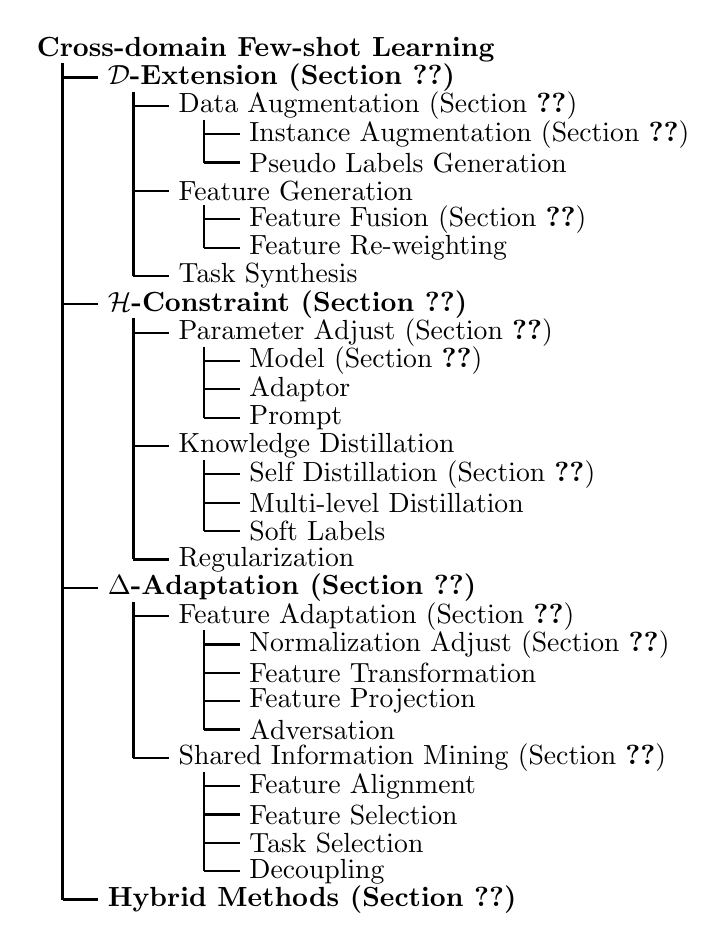
\begin{tikzpicture}[xscale=0.9, yscale=0.36]
\textcolor{black}{
\draw [thick, -] (0, 24) -- (0, 24); \node [right] at (-0.5, 24) {\textbf{Cross-domain Few-shot Learning
}};
\draw [thick, -] (0, 23.5) -- (0, -6);
\draw [thick, -] (0, 23) -- (0.5, 23);\node [right] at (0.5, 23) {\textbf{$\mathcal{D}$-Extension (Section~\ref{instance})}};
\draw [thick, -] (1, 22.5) -- (1, 16);
\draw [thick, -] (1, 22) -- (1.5, 22);\node [right] at (1.5, 22) {Data Augmentation (Section~\ref{sec:FSCIC:dba})};
\draw [thick, -] (2, 21.5) -- (2,20);
\draw [thick, -] (2, 21) -- (2.5, 21);\node [right] at (2.5, 21) {Instance Augmentation (Section~\ref{sec:FSCIC:dba:drbm})};
%\draw [thick, -] (2, 20.5) -- (2,19);
\draw [thick, -] (2, 20) -- (2.5, 20);\node [right] at (2.5, 20) {Pseudo Labels Generation};
\draw [thick, -] (1, 19) -- (1.5, 19);\node [right] at (1.5, 19) {Feature Generation
};
\draw [thick, -] (2, 18.5) -- (2,17);
\draw [thick, -] (2, 18) -- (2.5, 18);\node [right] at (2.5, 18) {Feature Fusion (Section~\ref{sec:FSCIC:dba:drbm})};
%\draw [thick, -] (2, 20.5) -- (2,19);
\draw [thick, -] (2, 17) -- (2.5, 17);\node [right] at (2.5, 17) {Feature Re-weighting};
\draw [thick, -] (1, 16) -- (1.5, 16);\node [right] at (1.5, 16) {Task Synthesis
};
\draw [thick, -] (0, 15) -- (0.5, 15);\node [right] at (0.5, 15) {\textbf{$\mathcal{H}$-Constraint (Section~\ref{hypothesis})}};
\draw [thick, -] (1, 14.5) -- (1, 6);
\draw [thick, -] (1, 14) -- (1.5, 14);\node [right] at (1.5, 14) {Parameter Adjust (Section~\ref{sec:FSCIC:dba})};
\draw [thick, -] (2, 13.5) -- (2,11);
\draw [thick, -] (2, 13) -- (2.5, 13);\node [right] at (2.5, 13) {Model (Section~\ref{sec:FSCIC:dba:drbm})};
%\draw [thick, -] (2, 20.5) -- (2,19);
\draw [thick, -] (2, 12) -- (2.5, 12);\node [right] at (2.5, 12) {Adaptor};
\draw [thick, -] (2, 11) -- (2.5, 11);\node [right] at (2.5, 11) {Prompt};
\draw [thick, -] (1, 10) -- (1.5, 10);\node [right] at (1.5, 10) {Knowledge Distillation
};
\draw [thick, -] (2, 9.5) -- (2,7);
\draw [thick, -] (2,9) -- (2.5, 9);\node [right] at (2.5, 9) {Self Distillation (Section~\ref{sec:FSCIC:dba:drbm})};
%\draw [thick, -] (2, 20.5) -- (2,19);
\draw [thick, -] (2, 8) -- (2.5, 8);\node [right] at (2.5, 8) {Multi-level Distillation};
\draw [thick, -] (2, 7) -- (2.5, 7);\node [right] at (2.5, 7) {Soft Labels};
\draw [thick, -] (1, 6) -- (1.5, 6);\node [right] at (1.5, 6) {Regularization
};
\draw [thick, -] (0, 5) -- (0.5, 5);\node [right] at (0.5, 5) {\textbf{$\Delta$-Adaptation (Section~\ref{adaptation})}};
\draw [thick, -] (1, 4.5) -- (1, -1);
\draw [thick, -] (1, 4) -- (1.5, 4);\node [right] at (1.5, 4) {Feature Adaptation (Section~\ref{sec:FSCIC:dba})};
\draw [thick, -] (2, 3.5) -- (2,0);
\draw [thick, -] (2, 3) -- (2.5, 3);\node [right] at (2.5, 3) {Normalization Adjust (Section~\ref{sec:FSCIC:dba:drbm})};
%\draw [thick, -] (2, 20.5) -- (2,19);
\draw [thick, -] (2, 2) -- (2.5, 2);\node [right] at (2.5, 2) {Feature Transformation};
\draw [thick, -] (2, 1) -- (2.5, 1);\node [right] at (2.5, 1) {Feature Projection};
\draw [thick, -] (2, 0) -- (2.5, 0);\node [right] at (2.5, 0) {Adversation
};
%\draw [thick, -] (2, -0.5) -- (2,-2);
\draw [thick, -] (1,-1) -- (1.5, -1);\node [right] at (1.5, -1) {Shared Information Mining (Section~\ref{sec:FSCIC:dba:drbm})};
\draw [thick, -] (2, -1.5) -- (2,-5);
\draw [thick, -] (2, -2) -- (2.5, -2);\node [right] at (2.5, -2) {Feature Alignment};
\draw [thick, -] (2, -3) -- (2.5, -3);\node [right] at (2.5, -3) {Feature Selection};
\draw [thick, -] (2, -4) -- (2.5, -4);\node [right] at (2.5, -4) {Task Selection};
\draw [thick, -] (2, -5) -- (2.5, -5);\node [right] at (2.5, -5) {Decoupling};
\draw [thick, -] (0, -6) -- (0.5, -6);\node [right] at (0.5, -6) {\textbf{Hybrid Methods (Section~\ref{hybrid})}};}
\end{tikzpicture}}
\vspace{-10pt}
\caption{\textcolor{black}{The taxonomy of representative methods in CDFSL.}}
\label{out}
\end{figure}
%\end{wrapfigure}
\fi
\section{Method}
\label{section:A}
\subsection{Overview}
Our goals are two-fold: 1) to promote the interpretability of the feature space for haze removal and 2) to establish a more concise solution space using of contrastive samples. Fig.~\ref{fig:method} illustrates the detailed structure of our C$^2$PNet. To achieve our first goal, we design a physics-aware dual-branch unit that is derived from the atmospheric scattering model. Regarding our second aim, we tailor a contrastive regularization using consensual negatives, along with a self-contained curriculum learning strategy to deal with the learning difficulty. Note that our curricular contrastive regularization is network-agnostic, making it applicable to other dehazing networks.
%\\
%\textbf{Physics-aware Dual-branch Unit.}
\subsection{Physics-aware Dual-branch Unit}
The atmospheric scattering model is commonly used to describe the formation of a hazy image $I$. It can be mathematically formulated as $I(x)=T(x)J(x)+(1-T(x))A$, where $J$ represents the clear image, $T$ is the transmission map, $A$ indicates the atmospheric light, and $x$ denotes the index of pixels. As both $T$ and $A$ are unknown, haze removal is a highly ill-posed problem. Raw space based methods directly estimate the two unknown factors, which can easily lead to cumulative errors. In contrast, imposing physics priors in the feature space can encourage the interpretability that aligns with the hazing process, without relying on the ground truths of $T$ and $A$. Inspired by FDU~\cite{dong2020physics}, we propose a physics-aware dual-branch Unit (PDU) that is derived from the physics model in the feature space, as shown in Fig.~\ref{fig:block}. 
\begin{figure}[t]
	\center
	\includegraphics[width=\linewidth]{fig/PDU.pdf}
	\caption{The architecture of the proposed PDU.}
	\label{fig:block}\vspace{-6mm}	
\end{figure}

To begin with, we reformulate the physics model to represent the clear image $J$ as follows:
\begin{equation}
	\begin{aligned}
		J(x)&=I(x)\frac{1}{T(x)}+A(1-\frac{1}{T(x)})\\
		&=I(x)\frac{1}{T(x)}+A-A\frac{1}{T(x)}.
	\end{aligned}
    \label{equ:scatter}
\end{equation}
Then extracting features via kernel $k$, Eq.~\eqref{equ:scatter} can be reformulated as follows:
\begin{equation}
	k\circledast J=k\circledast(I\odot\frac{1}{T})+k\circledast A-k\circledast(A\odot\frac{1}{T}), 
	\label{equ:conv}
\end{equation}
%Similar to the derivation in FDU, further
where $\circledast$ indicates the convolution operator and $\odot$ denotes the Hadamard product.  Consequently, we respectively introduce the matrix-vector forms of $k$, $J$, $I$, $A$, $\frac{1}{T}$, \ie, $\bm{K}$, $\bm{J}$, $\bm{I}$, $\bm{A}$ and $\bm{D}$, and Eq.~\eqref{equ:conv} can be rewritten as 
\begin{equation}
	\bm{KJ}=\bm{KDI}+\bm{KA}-\bm{KDA}.
\end{equation}
Such a reformulation can be given by a few steps of algebra operations. Note that the diagonal vector of the diagonal matrix $\bm{D}$ corresponds to the vectorized form of $\frac{1}{T}$.

Next, we can decompose the matrix $\bm{KD}$ into a product of two matrices $\bm{QK}$. As $\bm{K}$, $\bm{D}$ and $\bm{Q}$ are all unknown, implementing this decomposition can be indicated as solving an underdetermined system of equations, which can guarantee the existence of $\bm{Q}$. And then, we have
\begin{equation}	
	\bm{KJ}=\bm{Q}(\bm{KI})+\bm{KA}-\bm{Q}(\bm{KA}).
	\label{equ:Q}		
\end{equation}

We can denote $\tilde{\bm{A}}$ as an approximation of the features $\bm{KA}$ that correspond to the atmospheric light and $\tilde{\bm{t}}$ as an approximation of $\bm{Q}$, which is associated with the transmission map. Furthermore, $\bm{KI}$ and $\bm{KJ}$ can be viewed as the extracted features of a hazy image and its corresponding clear image, respectively. Based on Eq.~\eqref{equ:Q}, and assuming that the channel number of the features $\tilde{\bm{t}}$ matches that of the input features $\bm{M}$, we can calculate the physics-aware features $\tilde{\bm{J}}$ by 
\begin{equation}	
	\begin{aligned}
		\tilde{\bm{J}}&=\bm{M}\odot\tilde{\bm{t}}+\tilde{\bm{A}}-\tilde{\bm{A}}\odot\tilde{\bm{t}}\\		&=\bm{M}\odot\tilde{\bm{t}}+\tilde{\bm{A}}(\bm{1}-\tilde{\bm{t}}),
	\end{aligned}
    \label{equ:final}
\end{equation}
where $\bm{1}$ indicates a matrix whose elements are all ones. 

Note that the second term on the right-hand side of Eq.~\eqref{equ:final} involves a synergistic action between $\tilde{\bm{A}}$ and $\tilde{\bm{t}}$ that is ignored by FDU. Then we can explicitly build the PDU based on Eq.~\eqref{equ:final}. One branch in PDU (see the upper part of Fig.~\ref{fig:block}) is used to produce $\tilde{\bm{A}}$. As the atmospheric light is usually assumed to be homogeneous, we use global average pooling (GAP($\cdot$)) to eliminate unnecessary information in the feature space. And $\tilde{\bm{A}}$ is produced by
\begin{equation}	
	\tilde{\bm{A}}=H(\sigma(\textrm{Conv}^N(\textrm{ReLU}(\textrm{Conv}^{\frac{N}{8}}(\textrm{GAP}(\bm{M})))))),		
\end{equation}
where $\sigma(\cdot)$ is the Sigmoid function, $H(\cdot)$ denotes a replication operation, $\textrm{Conv}^N(\cdot)$ is the convolutional layer with $N$ kernels, and $N$ is set to 64.

On the other hand, we cannot apply GAP$(\cdot)$ for the approximation of $\bm{Q}$ due to a loss of information, as the transmission map is non-homogeneous. Therefore, in the lower branch in Fig.~\ref{fig:block}, we choose to extract $\tilde{\bm{t}}$ using a sequence of convolutional layers, which is given by
\begin{equation}	
	\tilde{\bm{t}}=\sigma(\textrm{Conv}^N(\textrm{ReLU}(\textrm{Conv}^{\frac{N}{8}}(\textrm{Conv}^{N}(\bm{M}))))).		
\end{equation}

With the proposed PDU, interpretable features $\tilde{\bm{J}}$ can be generated from the input features $\bm{M}$ for restoring hazy images. Unlike FDU, which uses a shared structure with GAP$(\cdot)$ to predict latent features that are simultaneously correlated to both $T$ and $A$, the PDU attentively incorporates the corresponding physical characteristics of these two factors. This approach allows for more useful features to be estimated in a dual interactive paradigm. 

%\textbf{Curricular Contrastive Regularization.}
\subsection{Curricular Contrastive Regularization} 
Regarding the canonical contrastive regularization for image dehazing, the anchor is the recovered result by the dehazing network, the positive is the ground truth, and the negatives include a hazy input and multiple hazy images that are non-consensual with the positive. The target of this regularization $R$ is to minimize the L1 distance between the embeddings of the anchor and the positive while maximizing their distance from the negatives, which is given by
\begin{equation}
	R=\sum_{i=1}^n\xi_i\frac{||V_i(J)-V_i(f(I,\theta))||_1}{\sum_{q=1}^r||V_i(U_q)-V_i(f(I,\theta))||_1+E_i},		
\end{equation}
where $E_i=||V_i(I)-V_i(f(I,\theta))||_1$, $f(\cdot,\theta)$ indicates the dehazing network with parameters $\theta$, $V_i(\cdot), i=1,2,\cdots,n$ extracts the $i$th hidden features from the pre-trained VGG-19~\cite{simonyan2014very}, the number of non-consensual negatives $\{U_q\}$ is $r$, and $\{\xi_{i}\}$ is the set of hyperparameters. As illustrated in Fig.~\ref{fig:CC}, the introduced contrast between the anchor and non-consensual negatives cannot provide a satisfactory lower bound of the solution space. The non-consensual negatives are typically distantly located from the positive, leading to an under-constricted solution space that limits the quality of the restorations.

Based on our analysis of Fig.~\ref{fig:teaser}, we propose a novel contrastive regularization for haze removal that utilizes negatives in the consensual space, which can be restored results from other dehazing models. Our straightforward aim is to push the anchor far away from better-quality negatives. However, two critical problems arise: 1) how to define the difficulty of different negatives and 2) how to arrange these negatives according to their difficulty during training. 
\begin{figure}[t]
	\center
	\includegraphics[width=\linewidth]{fig/CC.pdf}
	\caption{Illustration of curricular contrastive regularization.}
	\label{fig:CC}\vspace{-4mm}
\end{figure}

To solve both issues, we incorporate a curriculum learning strategy into contrastive regularization. We define the difficulty of the negatives into three levels: easy, hard, and ultra-hard. For easy negative, we use the hazy input consistently. The difficulty levels of the other negatives are dynamically determined during training. Specifically, we measure the average PSNR performance of the network before every epoch begins. In the $t$th epoch, a negative is defined as an ultra-hard sample when its PSNR is higher than the network performance, or as a hard negative otherwise. 

To properly arrange these negatives, we weigh them differently according to their difficulty levels. First, the weight of easy negative is fixed and largest. This is because although hard and ultra-hard negatives may contribute to a more compact solution space, they can also cause learning ambiguity. To ensure that the resultant force is towards the positive such that the anchor is shifted in the desired direction, we give the easy negative a weight that is large enough. In practice, we set this weight to the number of the non-easy negatives $z$. Second, the weight of a non-easy negative $S_q$ at the $t$th epoch is defined as follows: 
\begin{small}
\begin{equation}
	W_t(S_q) = \left\{
	\begin{array}{rcl}
		1+\gamma, &\textrm{avgPSNR}(f(\{I_g\},\theta_{t-1}))\geq \textrm{PSNR}(S_q),\\
		1-\gamma, & \textrm{otherwise},\\
	\end{array} \right. 
	\label{equ:beta}
\end{equation}
\end{small}
where $\{I_g\}$ denotes the hazy input dataset, $q=1,2,\cdots,z$ is the index of the non-easy negatives, and $\gamma$ is a hyperparameter. The weights of the hard and the ultra-hard negatives are set to $1+\gamma$ and $1-\gamma$, respectively. This means that the weight of a hard negative is larger than that of an ultra-hard negative, allowing the hard negative to provide a greater force and alleviating the potential learning ambiguity. Furthermore, the flexibility of this strategy in determining the difficulty levels enables ultra-hard negatives to become hard ones in the later stage of training (see Fig.~\ref{fig:CC}). This makes sense because as the quality of the anchor improves, the ambiguity caused by ultra-hard samples is reduced, and their importance should be strengthened. In this way, the hard and ultra-hard negatives can be viewed as better lower bounds for effectively constraining the solution space. Then, our curricular contrastive regularization $R^*$is formulated as follows:
\begin{small}
\begin{equation}
	R^*=\sum_{i=1}^n\xi_i\frac{||V_i(J)-V_i(f(I,\theta))||_1}{\sum_{q=1}^zW_t(S_q)||V_i(S_q)-V_i(f(I,\theta))||_1+z\cdot E_i}.
	\label{equ:R}	
\end{equation}
\end{small}

Finally, our total objective $\cal L$, which consists of an L1 norm based fidelity term and our contrastive curricular regularization, is given by
\begin{equation}
	{\cal L}=||J-f(I,\theta)||_1+\lambda R^*.	
\end{equation}
%\\


\subsection{Network Architecture}
\begin{table*}[t]
	\caption{Quantitative Evaluations with the state-of-the-art methods on the synthetic and real-world datasets.}
	\centering
	\small
	\begin{tabular}{c||c||c|c||c|c||c|c||c|c||c}
		\toprule
		\multirow{2}*{Method} &\multirow{2}*{Venue\&Year}&\multicolumn{2}{c||}{SOTS-indoor} &\multicolumn{2}{c||}{SOTS-outdoor} &\multicolumn{2}{c||}{Dense-Haze} &\multicolumn{2}{c||}{NH-Haze2} &\multirow{2}*{\#Params} \\
		\cmidrule(lr){3-4}
		\cmidrule(lr){5-6}
		\cmidrule(lr){7-8}
		\cmidrule(lr){9-10}		
		&&PSNR&SSIM&PSNR&SSIM&PSNR&SSIM&PSNR&SSIM&\\
		\midrule
		DCP~\cite{he2010single}&TPAMI2010&16.62&0.8179&19.13&0.8148&11.01&0.4165&11.68&0.6475&-\\
		
		DehazeNet~\cite{cai2016dehazenet}&TIP2016&21.14&0.8472&22.46&0.8514&9.48&0.4383&11.77&0.6217&0.01M\\
		
		AODNet~\cite{li2017aod}&ICCV2017&19.06&0.8504&20.29&0.8765&12.82&0.4683&12.33&0.6311&0.002M\\	
		
		DM2F-Net~\cite{Deng2019}&ICCV2019&34.29&0.9728&34.50&0.9815&14.99&0.5640&20.46&0.8217&92.14M\\
		
		GCANet~\cite{chen2019gated}&WACV2019&30.06&0.9596&22.76&0.8887&12.62&0.4208&18.79&0.7729&0.70M\\
		
		GDN~\cite{liu2019griddehazenet}&ICCV2019&32.16&0.9836&30.86&0.9819&14.96&0.5326&19.26&0.8046&0.96M\\	
		
		MSBDN~\cite{dong2020multi}&CVPR2020&32.77&0.9812&34.81&0.9857&15.13&0.5551&20.11&0.8004&31.35M\\	
		
		FFA-Net~\cite{qin2020ffa}&AAAI2020&36.39&0.9886&33.57&0.9840&12.22&0.4440&20.00&0.8225&4.46M\\	
		
		AECR-Net~\cite{wu2021contrastive}&CVPR2021&37.17&0.9901&-&-&15.80&0.4660&20.68&0.8282&2.61M\\
		
		MAXIM-2S~\cite{tu2022maxim}&CVPR2022&38.11&0.9908&34.19&0.9846&-&-&-&-&14.1M\\	
		
		DeHamer~\cite{guo2022image}&CVPR2022&36.63&0.9881&35.18&0.9860&16.62&0.5602&19.18&0.7939&132.45M\\	
		
		UDN~\cite{hong2022uncertainty}&AAAI2022&38.62&0.9909&34.92&0.9871&-&-&-&-&4.25M\\		
		\midrule
		\textbf{C$^2$PNet}   &&\textbf{42.56}&\textbf{0.9954}&\textbf{36.68}&\textbf{0.9900}&\textbf{16.88}&\textbf{0.5728}&\textbf{21.19}&\textbf{0.8334}&7.17M\\		
		\bottomrule
	\end{tabular}
	\label{tab:quantitative}
\end{table*}
\begin{figure*}[t]
	\centering
	%	\footnotesize
	\setlength{\abovecaptionskip}{0cm}
	\setlength{\tabcolsep}{0.05em}
	\setlength{\fboxrule}{1pt}
	\setlength{\fboxsep}{0pt}
	\begin{tabular}{cccccccc}			   		
		PSNR / SSIM& $18.09 /  0.7459 $ & $31.55 / 0.9793$ & $34.41 / 0.9811$ & $36.69 / 0.9838$ & $37.10 / 0.9825$ & $41.20 / 0.9914$ & $\infty / 1$ \\			
		\includegraphics[width=.12\linewidth]{fig/indoor/rect/hazy.png} &
		\includegraphics[width=.12\linewidth]{fig/indoor/rect/aod.png} &
		\includegraphics[width=.12\linewidth]{fig/indoor/rect/gdn.png} &
		\includegraphics[width=.12\linewidth]{fig/indoor/rect/ffa.png} &
		\includegraphics[width=.12\linewidth]{fig/indoor/rect/maxim.png} &
		\includegraphics[width=.12\linewidth]{fig/indoor/rect/dehamer.png} &
		\includegraphics[width=.12\linewidth]{fig/indoor/rect/ours.png}&
		\includegraphics[width=.12\linewidth]{fig/indoor/rect/clear.png}\\	
		\fcolorbox{red}{red}{\includegraphics[width=.117\linewidth]{fig/indoor/crop/hazy.png}} &
		\fcolorbox{red}{red}{\includegraphics[width=.117\linewidth]{fig/indoor/crop/aod.png}} &
		\fcolorbox{red}{red}{\includegraphics[width=.117\linewidth]{fig/indoor/crop/gdn.png}} &
		\fcolorbox{red}{red}{\includegraphics[width=.117\linewidth]{fig/indoor/crop/ffa.png}}&
		\fcolorbox{red}{red}{\includegraphics[width=.117\linewidth]{fig/indoor/crop/maxim.png}} &
		\fcolorbox{red}{red}{\includegraphics[width=.117\linewidth]{fig/indoor/crop/dehamer.png}}&
		\fcolorbox{red}{red}{\includegraphics[width=.117\linewidth]{fig/indoor/crop/ours.png}}&
		\fcolorbox{red}{red}{\includegraphics[width=.117\linewidth]{fig/indoor/crop/clear.png}}\\
		Hazy Image &AODNet~\cite{li2017aod}&GDN~\cite{liu2019griddehazenet}&FFA-Net~\cite{qin2020ffa}&MAXIM~\cite{tu2022maxim}&DeHamer~\cite{guo2022image}&C$^2$PNet (Ours)&GT
	\end{tabular}
	\caption{Visual results of SOTS-indoor dataset by different methods. (Zoom in for better view.)
	}
	\label{fig:indoor}
\end{figure*}

Our C$^2$PNet adopts an FFA-Net-like backbone because: 1) FFA-Net has a simple structure that cascades several FA blocks without any other redundant modules, and 2) the FA block is simple and has been proven to be practical. Since the proposed PDU mainly focuses on refining spatial information, we deploy it into each FA block by replacing the PA module. In this way, the features are enforced to conform to the hazing process before being fed into the subsequent module. Note that all other network parameters of C$^2$PNet are identical to those of FFA-Net, except for the PDUs.



\section{Datasets}
We use PURE~\cite{Stricker2014}, UBFC-rPPG~\cite{Bobbia2019}, and DDPM~\cite{Speth_IJCB_2021} as benchmark rPPG datasets for training and testing, and CelebV-HQ dataset~\cite{zhu2022celebvhq} and HKBU-MARs~\cite{Liu_2016_CVPRW} for unsupervised training only.

\noindent
\textbf{ Deception Detection and Physiological Monitoring (DDPM)}~\cite{Speth_IJCB_2021,Vance2022} consists of 86 subjects in an interview setting, where subjects attempted to answer questions deceptively. Interviews were recorded at 90 frames-per-second for more than 10 minutes on average. Natural conversation and frequent head pose changes make it a difficult and less-constrained rPPG dataset.

%\noindent
\textbf{PURE}~\cite{Stricker2014} is a benchmark rPPG dataset consisting of 10 subjects recorded over 6 sessions. Each session lasted approximately 1 minute, and raw video was recorded at 30 fps. The 6 sessions for each subject consisted of: (1) steady, (2) talking, (3) slow head translation, (4) fast head translation, (5) small and (6) medium head rotations. Pulse rates are at or close to the subject's resting rate.

%\noindent
\textbf{UBFC-rPPG}~\cite{Bobbia2019} contains 1-minute long videos from 42 subjects recorded at 30 fps. Subjects played a time-sensitive mathematical game to raise their heart rates, but head motion is limited during the recording.

%\noindent
\textbf{HKBU 3D Mask Attack with Real World Variations (HKBU-MARs)}~\cite{Liu_2016_CVPRW} consists of 12 subjects captured over 6 different lighting configurations with 7 different cameras each, resulting in 504 videos lasting 10 seconds each. The diverse lighting and camera sensors make it a valuable dataset for unsupervised training. We use version 2 of HKBU-MARs, which contains videos with both realistic 3D masks and unmasked subjects.

%\noindent
\textbf{High-Quality Celebrity Video Dataset (CelebV-HQ)}~\cite{zhu2022celebvhq} is a set of processed YouTube videos containing 35,666 face videos from over 15,000 identities. The videos vary dramatically in length, lighting, emotion, motion, skin tones, and camera sensors. The greatest challenge in harnessing online videos is their reduced quality due to compression before upload and by the video provider. Compression is a known challenge for rPPG, since the blood volume pulse is so subtle optically~\cite{McDuff2017,Nowara_ICCVW_2019,Rapczynski2019,Nowara_BOE_2021}.
\section{Training Details}

\setlength\tabcolsep{4pt}
\begin{table*}[htb!]
\caption{{\bf Intra-dataset} pulse rate estimation results. The best results for a given metric/dataset are bolded, and the second-best results are underlined. For a better comparison with results in the literature, this table follows \cite{Sun_2022_ECCV}. MAE: Mean Absolute Error; RMSE: Root Mean Square Error; $r$: Pearson correlation coefficient.}
\fontsize{7.533}{9}\selectfont
% \tiny
\centering
% \setlength{\tabrowsep}{1mm}
{
\begin{threeparttable}
\begin{tabular}{llccccccccc}
% \begin{tabular}{llrrrrrrrrr}
% \begin{tabular}{lllllllllll}
\toprule
\multirow{2}{*}{\begin{tabular}[c]{@{}l@{}}\\ Types\end{tabular}} &
\multirow{2}{*}{\begin{tabular}[c]{@{}l@{}}\\Methods\end{tabular}} &
\multicolumn{3}{c}{UBFC-rPPG} & \multicolumn{3}{c}{PURE} &
\multicolumn{3}{c}{DDPM} \\ 
\cmidrule(lr){3-5}\cmidrule(lr){6-8}\cmidrule(lr){9-11}
& & \begin{tabular}[c]{@{}c@{}}MAE\\ (bpm)\end{tabular} & \begin{tabular}[c]{@{}c@{}}RMSE\\ (bpm)\end{tabular} & $r$                    & \begin{tabular}[c]{@{}c@{}}MAE\\ (bpm)\end{tabular} & \begin{tabular}[c]{@{}c@{}}RMSE\\ (bpm)\end{tabular} & $r$                    & \begin{tabular}[c]{@{}c@{}}MAE\\ (bpm)\end{tabular} & \begin{tabular}[c]{@{}c@{}}RMSE\\ (bpm)\end{tabular} & $r$                  \\ 
\midrule
% \multirow{5}{*}{\begin{tabular}[c]{@{}l@{}}Tradi-\\tional\end{tabular}}
\multirow{5}{*}{\rot{Traditional}}
& GREEN \cite{Verkruysse2008} & 7.50 & 14.41 & 0.62 & 7.23 & 17.05 & 0.69 & 32.79 & 43.09 & 0.04 \\
& ICA \cite{Poh2011} & 5.17 & 11.76 & 0.65 & 3.76 & 12.60 & 0.85 & 22.22 & 35.77 & 0.40 \\
& CHROM \cite{DeHaan2013} &
    2.36 & 9.23 & 0.87 &
    \underline{0.75} & 2.23 & \bf 1.00 &
    13.48 & 28.53 & 0.56 \\
& 2SR \cite{Wang2016} & - & - & - &
    2.44 & 3.06 & 0.98 & - & - & - \\
& POS \cite{Wang2017} &
    2.11 & 9.11 & 0.87 &
    0.80 & 4.11 & 0.98 &
    9.03 & 23.07 & 0.70 \\
 
\midrule
\multirow{6}{*}{\rot{Supervised}}

& HR-CNN \cite{Spetlik_2018} & - & - & - & 1.84 & 2.37 & 0.98 & - & - & - \\
& SynRhythm \cite{Niu2018} & 5.59 & 6.82 & 0.72 & - & - & - & - & - & - \\
& PulseGAN \cite{Song_2021} & 1.19 & 2.10 & \underline{0.98} & - & - & - & - & - & - \\
& Dual-GAN \cite{Lu_2021} &
    \bf{0.44} & \bf{0.67} & \bf{0.99} &
    0.82 & \bf{1.31} & \underline{0.99} &
    - & - & - \\
& RPNet \cite{Speth_CVIU_2021}\tnote{\textdagger} &
    \underline{0.53 $\pm$ 0.01} & 1.78 $\pm$ 0.02 & \bf{0.99 $\pm$ 0.00} &
    1.15 $\pm$ 0.27 & 5.77 $\pm$ 1.25 & 0.96 $\pm$ 0.02 &
    \bf 3.46 $\pm$ 0.24 & \bf 12.47 $\pm$ 0.68 & \bf 0.91 $\pm$ 0.01 \\
& PhysNet \cite{Yu2019}\tnote{\textdagger} &
    0.55 $\pm$ 0.03 & 2.03 $\pm$ 0.37 & \bf 0.99 $\pm$ 0.00 &
    0.99 $\pm$ 0.19 & 5.22 $\pm$ 0.93 & 0.97 $\pm$ 0.01 &
    \underline{3.96 $\pm$ 0.76} & \underline{13.57 $\pm$ 1.74} & 
    \underline{0.89 $\pm$ 0.03} \\
\midrule


\multirow{5}{*}{\rot{Unsupervised}}
 & Gideon2021 \cite{Gideon_2021_ICCV} & 
    1.85 & 4.28 & 0.93 &
    2.3 & 2.9 & \underline{0.99} &
    - & - & - \\
 & SLF-RPM~\cite{Wang_SSL_2022}\tnote{*} &
    8.39 & 9.70 & 0.70 &
    - & - & - &
    - & - & - \\
 & SimPer~\cite{Yuzhe_SimPer_2022}\tnote{*} &
    4.24 & - & - &
    3.89 & - & - &
    - & - & - \\
 & Contrast-Phys~\cite{Sun_2022_ECCV} &
    0.64 & \underline{1.00} & \bf{0.99} &
    1.00 & \underline{1.40} & \underline{0.99} &
    9.70 $\pm$ 2.90 & 25.02 $\pm$ 6.01 & 0.58 $\pm$ 0.19 \\
 & \bf{\ourapproach (ours)} &
    0.59 $\pm$ 0.00 & 1.83 $\pm$ 0.04 & \bf 0.99 $\pm$ 0.00 &
    \bf 0.61 $\pm$ 0.06 & 1.84 $\pm$ 0.40 & \bf 1.00 $\pm$ 0.00 &
    5.87 $\pm$ 0.11 & 17.44 $\pm$ 0.16 & 0.81 $\pm$ 0.00 \\
\bottomrule
\end{tabular}
\begin{tablenotes}\footnotesize
        % \vspace{0.1ex}
        \item[*] Some methods in the unsupervised row require fine-tuning on labeled data with a linear classifier.
        \item[\textdagger] Some supervised methods were trained with identical data augmentations to \ourapproach for fair comparison.
        \end{tablenotes}
    \end{threeparttable}
}
\label{tab:within_dataset}
\end{table*}

\subsection{Data Preprocessing}
To prepare the video clips for the spatiotemporal deep learning models, we first extract 68 face landmarks with OpenFace~\cite{Baltrusaitis2018}. We then define a bounding box in each frame with the minimum and maximum $(x,y)$ locations by extending the crop horizontally by 5\% to ensure that the cheeks and jaw are present. The top and bottom are extended by 30\%  and 5\% of the bounding box height, respectively, to include the forehead and jaw. We further extend the shorter of the two axes to the length of the other to form a square. The cropped frames are then resized to 64$\times$64 pixels with bicubic interpolation. For faster processing of the massive CelebV-HQ~\cite{zhu2022celebvhq} dataset, we instead use MediaPipe Face Mesh~\cite{lugaresi2019mediapipe} for landmarking.


\subsection{Model Architectures}
We use a 3D-CNN architecture similar to \cite{Speth_CVIU_2021} without temporal dilations, which was originally inspired by \cite{Yu2019}. We use a temporal kernel width of 5, and replace default zero-padding by repeating the edges. Zero-padding along the time dimension can result in edge effects that add artificial frequencies to the predictions. Early experiments showed that temporal dilations caused aliasing and reduced the bandwidth of the model to specific frequencies. Our losses and framework may be applied to any task and architecture with dense predictions along one or more dimensions. However, popular rPPG architectures such as DeepPhys~\cite{Chen2018} and  MTTS-CAN~\cite{Liu_MTTS_2020} may be ill-suited for the approach, since they consume very few frames, and the number of time points should be large enough to give sufficient frequency resolution with the FFT. In our experiments, we use the AdamW~\cite{Loshchilov2019AdamW} optimizer with a learning rate of 0.0001. We use a clip length of $T=120$ frames (4 seconds), and we set the input signal’s length to achieve a frequency resolution of $0.\overline{33}$ bpm.

\subsection{Supervised Training}
To properly compare our approach to its supervised counterpart we use the same model architecture and train it with the commonly used negative Pearson loss between the predicted waveform and the contact sensor ground truth~\cite{Yu2019}. During training we apply all of the same augmentations except time reversal. Models are trained for 200 epochs on PURE and UBFC-rPPG, and for 40 epochs on DDPM. The model from the epoch with the lowest loss on the validation set is selected for testing.

\subsection{Unsupervised Training}
Unsupervised models are trained for the same number of epochs as the supervised setting for both PURE and UBFC-rPPG, but we train for an additional 40 epochs on DDPM, since this dataset is considerably more difficult. We set the batch size to 20 samples during training. Contrary to previous unsupervised approaches~\cite{Gideon_2021_ICCV,Sun_2022_ECCV}, we leverage validation sets for model selection by selecting the model with the lowest combined bandwidth and sparsity losses. The creation of the dataset splits is described in the next section.

\subsection{Evaluation}
Pulse rates are computed as the highest spectral peak between 0.66 Hz and 3 Hz (equivalent to 40 bpm to 180 bpm) over a 10-second sliding window. The same procedure is applied to the ground truth waveforms for a reliable evaluation~\cite{Mironenko2020}. We apply common error metrics such as mean absolute error (MAE), root mean square error (RMSE), and Pearson correlation coefficient ($r$) between the pulse rates.

We perform 5-fold cross validation for both PURE and UBFC with the same folds as \cite{Gideon_2021_ICCV}, and use the predefined dataset splits from DDPM~\cite{Speth_CVIU_2021}. Differently from \cite{Gideon_2021_ICCV}, we use 3 of the folds for training, 1 for validation, and the remaining for testing rather than only training and testing partitions. We train 3 models with different initializations, resulting in 15 models trained on PURE and UBFC each, and 3 models trained on DDPM. We present the mean and standard deviation of the errors in the results.
\section{Results}
\subsection{Within-Dataset Testing}
Table \ref{tab:within_dataset} shows the results for models trained and tested on subject-disjoint partitions from the same datasets. For PURE and UBFC we achieve MAE lower than 1 bpm, performing better or on par with all traditional and supervised learning approaches. For PURE, our approach gives the lowest MAE and a Pearson $r$ of nearly 1. Performance drops on DDPM due to the overall difficulty of the dataset. \ourapproach outperforms contrastive approaches, only being surpassed by supervised deep learning models.

In comparison to other unsupervised methods, Contrast-Phys~\cite{Sun_2022_ECCV} gives the most competitive performance on all but DDPM. Note that our approach gives the lowest MAE on all datasets, but has higher RMSE. We believe this is due their use of harmonic removal as a post-processing step when estimating the pulse rate, which is not described in \cite{Sun_2022_ECCV}, but can be found in their publicly available code. 

\subsection{Cross-Dataset Testing}
\begin{table}[!htb]
\setlength\tabcolsep{6pt}
\centering\footnotesize
\caption{{\bf Cross-dataset} pulse rate estimation performance. The top 3 training datasets are common rPPG benchmarks, while HKBU was not designed for rPPG and has no pulse ground truth. Note that testing on UBFC after training on DDPM performs well, since their frequency distributions are similar, while PURE's pulse rates tend to be much lower.}
%\begin{tabular}{ccccc}
\begin{tabular}{cccrr}
\toprule
% \begin{tabular}{@{}c@{}}\textbf{Dataset}\\\textbf{Type}\end{tabular} &
\begin{tabular}{@{}c@{}}\textbf{Training}\\\textbf{Dataset}\end{tabular} & \begin{tabular}{@{}c@{}}\textbf{Testing}\\\textbf{Dataset}\end{tabular} & {\bf Method} & \begin{tabular}{@{}c@{}}{\bf MAE\phantom{xxi}}\\\textbf{(bpm)\phantom{xxi}}\end{tabular} & {\bf $r$\phantom{xxxx}}
\\
\cmidrule{1-5}
% \multirow{4}{*}{\underline{DDPM}}
\multirow{6}{*}{DDPM}
& UBFC & \ourapproach & 0.88 $\pm$ 0.25 & 0.98 $\pm$ 0.01\\
& UBFC & Contrast-Phys & 1.14 $\pm$ 0.38 & 0.96 $\pm$ 0.03\\
& UBFC & PhysNet & 1.11 $\pm$ 0.42 & 0.95 $\pm$ 0.02 \\
\cline{2-5}\\[-2ex]
& PURE & \ourapproach & 3.12 $\pm$ 1.07 & 0.88 $\pm$ 0.05 \\
& PURE & Contrast-Phys & 13.02 $\pm$ 6.12 & 0.19 $\pm$ 0.59  \\
& PURE & PhysNet & 1.46 $\pm$ 0.34 & 0.95 $\pm$ 0.02 \\
% \cline{2-5}\\[-2ex]
\midrule
 
\multirow{6}{*}{UBFC}
& DDPM & \ourapproach & 18.53 $\pm$ 0.36 & 0.38 $\pm$ 0.01 \\
& DDPM & Contrast-Phys & 22.93 $\pm$ 1.02 & 0.18 $\pm$ 0.04 \\
& DDPM & PhysNet & 18.58 $\pm$ 0.12 & 0.40 $\pm$ 0.00 \\
\cline{2-5}\\[-2ex]
& PURE & \ourapproach & 4.02 $\pm$ 0.06 & 0.86 $\pm$ 0.00 \\
& PURE & Contrast-Phys & 19.61 $\pm$ 2.01 & 0.33 $\pm$ 0.06 \\
& PURE & PhysNet & 3.81 $\pm$ 0.34 & 0.87 $\pm$ 0.02 \\
\midrule

\multirow{6}{*}{PURE}
& UBFC & \ourapproach & 6.64 $\pm$ 1.76 & 0.59 $\pm$ 0.10 \\
& UBFC & Contrast-Phys & 10.22 $\pm$ 0.38 & 0.45 $\pm$ 0.04 \\
& UBFC & PhysNet & 7.02 $\pm$ 3.35 & 0.60 $\pm$ 0.13 \\
\cline{2-5}\\[-2ex]
& DDPM & \ourapproach & 24.92 $\pm$ 0.65 & 0.20 $\pm$ 0.00 \\
& DDPM & Contrast-Phys & 29.63 $\pm$ 0.48 & 0.03 $\pm$ 0.02 \\
& DDPM & PhysNet & 28.03 $\pm$ 2.20 & 0.13 $\pm$ 0.05\\
% \bottomrule\\[-1.5ex]
\midrule
\midrule

% \multirow{3}{*}{\begin{tabular}{@{}c@{}}\underline{HKBU}\\\underline{(non-rPPG)}\end{tabular}}
\multirow{3}{*}{\begin{tabular}{@{}c@{}}HKBU\\(non-rPPG)\end{tabular}}

& UBFC & \ourapproach &  1.08 $\pm$ 0.03 & 0.95 $\pm$ 0.00 \\
& PURE      & \ourapproach &  2.43 $\pm$ 0.20 & 0.90 $\pm$ 0.02 \\
& DDPM      & \ourapproach & 20.34 $\pm$ 0.25 & 0.19 $\pm$ 0.02 \\
\bottomrule
\end{tabular}
\label{tab:cross_dataset}
\end{table}

We perform cross-dataset testing to analyze whether the approach is robust to changes to the lighting, camera sensor, pulse rate distribution, and motion. Table \ref{tab:cross_dataset} shows the results for \ourapproach and supervised training with the same architecture. We find that the performance is similar for the supervised and unsupervised approaches when transferring to different data sources. Training on PURE exclusively gives relatively poor results when transferring to UBFC-rPPG and DDPM, due to the low pulse rate variability within PURE samples and lack of movement. Training on DDPM gives the best results overall, since the dataset is the largest and captures larger subjects' movements compared to other datasets.

\subsection{Training with CelebV-HQ Videos}\label{sec:celebv_training}
Given the abundance of face videos publicly available online, we trained a model on the CelebV-HQ dataset~\cite{zhu2022celebvhq}. After processing the available videos with MediaPipe and resampling to 30 fps, our unlabeled dataset consisted of 34,029 videos. We trained the model for 23 epochs and manually stopped training due to a plateau in the validation loss.
Unfortunately, we found that the model could not converge to the true blood volume pulse. We attribute the failure to poor video quality from compression. Although the videos were downloaded with the highest available quality, they have likely been compressed multiple times, removing the pulse signal entirely. See Appendix \ref{sec:app_celebv} for a quantitative assessment of rPPG quality using a baseline approach.
%The MAE in bpm for UBFC-rPPG, PURE, and DDPM was 19.22, 24.83, and 27.41, respectively.

\subsection{Training with HKBU-MARs Videos}
The HKBU-MARs dataset~\cite{Liu_2016_CVPRW} was designed for face presentation attack detection, but we trained models on the ``real'' video sessions in the dataset. The bottom rows in Table \ref{tab:cross_dataset} show the results for training on HKBU-MARs, then testing on the benchmark rPPG datasets. Training on HKBU-MARs gives better results when testing on UBFC-rPPG and PURE than all training sets except DDPM, which is an order of magnitude larger. {\bf To our knowledge, this is the first succesful experiment showing that non-rPPG videos can be used to train robust rPPG models, even if they do not have ground-truth pulse labels}.

\begin{figure}
    \centering
    \includegraphics[width=\linewidth]{figures/waveforms.png}
    \caption{Within-dataset waveform predictions on all baseline datasets from end-to-end unsupervised models over an 8-second window. The model predictions are remarkably periodic without any form of filtering. Note that phase is not considered during training, so each model learns its own phase shift.}
    \label{fig:preds}
\end{figure}

\subsection{Ablation Study on Losses}
\begin{table}[!htb]
\setlength\tabcolsep{6pt}
\centering\footnotesize
\caption{Ablation study on the loss functions used during training. Results are shown for models trained and tested on UBFC-rPPG.}
\begin{tabular}{lrrr}
\toprule
{\bf Loss} & {\bf MAE (bpm)} & {\bf RMSE (bpm)} & {\bf $r$\phantom{xxxx}}
\\
\midrule
    $L_b$   &  3.08 $\pm$ 1.69 &  8.08 $\pm$ 3.61 &  0.87 $\pm 0.08$ \\
    $L_s$   & 45.50 $\pm$ 1.22 & 50.04 $\pm$ 0.94 & -0.04 $\pm 0.08$ \\
    $L_v$   & 22.89 $\pm$ 2.83 & 31.51 $\pm$ 2.36 &  0.22 $\pm 0.09$ \\
    $L_s+L_v$   & 51.24 $\pm$ 5.36 & 57.80 $\pm$ 7.39 & -0.04 $\pm 0.09$ \\
    $L_b+L_s$   &  9.99 $\pm$ 2.55 & 17.14 $\pm$ 2.36 &  0.51 $\pm 0.14$ \\
    $L_b+L_v$   &  4.18 $\pm$ 2.88 &  8.90 $\pm$ 5.24 &  0.82 $\pm 0.14$ \\
    \midrule
    \textbf{$L_b+L_s+L_v$}  & \bf 0.59 $\pm$ 0.00 & \bf 1.83 $\pm$ 0.04 & \bf 0.99 $\pm$ 0.00 \\
% \midrule
% \multirow{3}{*}{\underline{PURE}}
% & b   &  9.08 $\pm$ 2.16 & 18.56 $\pm$  2.34 & 0.66 $\pm$ 0.08 \\
% & s   & 22.10 $\pm$ 0.25 & 30.45 $\pm$  0.36 & 0.04 $\pm$ 0.02 \\
% & v   & 34.37 $\pm$ 3.61 & 44.71 $\pm$  3.62 & 0.14 $\pm$ 0.04 \\
% & sv  & 33.34 $\pm$ 7.79 & 48.78 $\pm$ 12.82 & 0.00 $\pm$ 0.01 \\
% & bs  & 13.44 $\pm$ 1.65 & 21.97 $\pm$  1.28 & 0.51 $\pm$ 0.07 \\
% & bv  &  9.99 $\pm$ 3.16 & 19.43 $\pm$  2.96 & 0.63 $\pm$ 0.10 \\
% & bsv &  4.02 $\pm$ 0.06 & 12.03 $\pm$  0.16 & 0.86 $\pm$ 0.00 \\
% \midrule
% \multirow{3}{*}{\underline{DDPM}}
% & b   & 22.25 $\pm$ 0.97 & 32.56 $\pm$ 0.83 &  0.26 $\pm$ 0.04 \\
% & s   & 47.38 $\pm$ 0.47 & 56.04 $\pm$ 0.41 & -0.01 $\pm$ 0.01 \\
% & v   & 34.04 $\pm$ 0.31 & 42.21 $\pm$ 0.50 &  0.02 $\pm$ 0.02 \\
% & sv  & 50.40 $\pm$ 2.48 & 59.79 $\pm$ 3.06 &  0.01 $\pm$ 0.01 \\
% & bs  & 23.76 $\pm$ 1.00 & 34.03 $\pm$ 0.71 &  0.21 $\pm$ 0.03 \\
% & bv  & 21.95 $\pm$ 1.57 & 32.12 $\pm$ 0.98 &  0.27 $\pm$ 0.06 \\
% & bsv & 18.53 $\pm$ 0.36 & 30.43 $\pm$ 0.41 &  0.38 $\pm$ 0.01 \\
\bottomrule
\end{tabular}
\label{tab:loss_ablation}
\end{table}
We trained models using all combinations of loss components to analyze their contributions. Table \ref{tab:loss_ablation} shows the results for training and testing on UBFC-rPPG. The bandwidth loss is the most critical for discovering the true blood volume pulse, while the sparsity and variance losses do not learn the desired signal by themselves. Surprisingly, combining the bandwidth loss with just one of the sparsity or variance losses gives worse performance than just the bandwidth loss. However, when combining all three components, the model achieves impressive results.
\section{Discussion}

\subsection{Improvements over Supervised Learning}
It is initially surprising that unsupervised training leads to similar or improved rPPG estimation models compared to those trained in a supervised manner. However, there are several potential benefits to unsupervised training. From a hardware perspective, one of the difficulties in supervised training is aligning the contact pulse waveform with the video frames~\cite{Zhan2020}. The pulse sensor and camera may have a time lag, effectively giving the model an out-of-phase target at training time. Unsupervised training gives the model freedom to learn the phase directly from the video. The contact-PPG signal is also sensitive to motion and may be noisy. Since motion may co-occur at the face and fingertip, the contact signal may misguide the model towards visual features for which they should be invariant.

From a physiological perspective, the pulse observed optically at the fingertip with a contact sensor has a different phase than that of the face, since blood propagates along a different path before reaching the peripheral microvasculature, making alignment nearly impossible without shifting the targets to rPPG estimates from existing methods~\cite{Speth_CVIU_2021}. Additionally, the morphological shape of the contact-PPG waveform depends on numerous factors such as the wavelength of light (and corresponding tissue penetration depth), external pressure from the oximeter clip, and vasodilation at the measurement site~\cite{Moco2018,Abraham2013}. This indicates that the morphology and phase of the target PPG waveform is likely different from the observed rPPG waveform.

\subsection{Why Does It Work?}
The success of the proposed non-contrastive approach depends on specific properties of the data, model, and how the two interact.
Limited model capacity is actually a strength, since it forces discovering features to generalize across inputs.
An infinite capacity network could discover spurious signals in the training data and fail to generalize.
By constraining the model's predictions to have specific periodic properties the limited-capacity model must find a general set of features to produce a signal that exists in all of the training samples, which happens to be the blood volume pulse in our datasets.

As a beneficial side-effect, the model intrinsically learns to ignore common noise factors such as illumination, rigid motion, non-rigid motion (\eg talking, smiling, etc.), and sensor noise, since they may preside outside the predefined bandlimits or with uniform power spectra.
Even if noise exhibits periodic tendencies within the bandlimits for some samples, those features would produce poor signals on other samples.
Therefore, end-to-end unsupervised approaches are particularly well-suited for periodic problems.


\section{Conclusions}
We proposed a novel non-contrastive learning approach for end-to-end unsupervised signal regression, with specific experiments on blood volume pulse estimation from face videos.
This SiNC framework effectively learns powerful visual features with only loose frequency constraints.
We demonstrated this by training accurate rPPG models using non-rPPG data and our simple loss functions.
Given the subtlety of the rPPG signal, we believe our work can be extended to other signal regression tasks in the domain of remote vitals estimation.
\section*{Acknowledgements}
This research was sponsored by the Securiport Global Innovation Cell, a division of Securiport LLC. Commercial equipment is identified in this work in order to adequately specify or describe the subject matter. In no case does such identification imply recommendation or endorsement by Securiport LLC, nor does it imply that the equipment identified is necessarily the best available for this purpose. The opinions, findings, and conclusions or recommendations expressed in this publication are those of the authors and do not necessarily reflect the views of our sponsors.

%%%%%%%%% REFERENCES
{\small
\bibliographystyle{ieee_fullname}
\bibliography{biblio}
}
\appendix

\section{Appendix for Proofs}

\paragraph{Proof of Theorem \ref{thm:main}.}

\begin{proof}
\label{proof:main}
Our proof has two steps. In Step 1, we will show that SimCLR is equivalent to minimizing the cross entropy loss defined in Eqn.~(\ref{eqn:cross-entropy}). 
In Step 2, we will show  that minimizing the cross-entropy loss 
is equivalent to spectral clustering on $\bfpi$. 
Combining the two steps together, we have proved our theorem. 

\textbf{Step 1: } SimCLR is equivalent to minimizing the cross entropy loss.

The cross-entropy loss takes expectation over 
$\bfW_\bfX\sim \mathbb{P}(\cdot ; \bfpi)$, 
which means $\bfW_\bfX$ has exactly one non-zero entry in each row $i$. By Lemma~\ref{lem:multinomial}, we know every row $i$ of $\bfW_\bfX$ is independent of other rows. Moreover, 
$\bfW_{\bfX,i}\sim \mathcal{M}(1, \bfpi_i/\sum_j \bfpi_{i,j})=\mathcal{M}(1, \bfpi_i)$, because $\bfpi_i$ itself is a probability distribution.
Similarly, we know $\bfW_\bfZ$ also has the row-independent property by sampling over $\mathbb{P}(\cdot;\bfK_\bfZ)$.
Therefore, by Lemma~\ref{lem:cross_split}, we know Eqn.~(\ref{eqn:cross-entropy}) is equivalent to:
\[
 -\sum_{i=1}^n \mathbb{E}_{\bfW_{\bfX,i}}[\log \mathbb{P}(\bfW_{\bfZ,i}=\bfW_{\bfX,i};\bfK_\bfZ)],
\]

This expression takes expectation over $\bfW_{\bfX,i}$ for the given row $i$. Notice that 
$\bfW_{\bfX,i}$ has exactly one non-zero entry, which equals $1$ (same for $\bfW_{\bfZ,i}$). 
As a result
we expand the above expression to be:
\begin{equation}
 -\sum_{i=1}^n \sum_{j\neq i} \Pr(\bfW_{\bfX,i,j}=1)\log \Pr(\bfW_{\bfZ,i,j}=1).
\label{eqn:detailed-expansion}    
\end{equation}


By Lemma~\ref{lem:multinomial}, $\Pr(\bfW_{\bfZ,i,j}=1)=\bfK_{\bfZ,i,j}/\|\bfK_{\bfZ,i}\|_1$ for $j\neq i$. Recall that $\bfK_\bfZ=(k(\bfZ_i-\bfZ_j))_{(i,j)\in[n]^2}$, which means 
$\bfK_{\bfZ,i,j}/\|\bfK_{\bfZ,i}\|_1=\frac{\exp(-\|\bfZ_i-\bfZ_j\|^2/{2\tau})}{\sum_{k\neq i}
\exp(-\|\bfZ_i-\bfZ_k\|^2/{2\tau})
}$ for $j\neq i$, when $k$ is the Gaussian kernel with variance $\tau$. 

Notice that $\bfZ_i=f(\bfX_i)$, so we know
\begin{equation}
-\log \Pr(\bfW_{\bfZ,i,j}=1)=
-\log \frac{\exp(-\|f(\bfX_i)-f(\bfX_j)\|^2/{2\tau})}{\sum_{k\neq i}
\exp(-\|f(\bfX_i)-f(\bfX_k)\|^2/{2\tau}),
}
\label{eqn:infonce-equivalence}    
\end{equation}


The right hand side is exactly the InfoNCE loss defined in Eqn.~(\ref{eqn:infonce}).
Inserting Eqn.~(\ref{eqn:infonce-equivalence}) into Eqn.~(\ref{eqn:detailed-expansion}), we get the SimCLR algorithm, which first samples augmentation pairs $(i,j)$ with $\Pr(\bfW_{\bfX,i,j}=1)$ for each row $i$, and then optimize the InfoNCE loss. 

\textbf{Step 2: } minimizing the cross entropy loss 
is equivalent to spectral clustering on $\bfpi$.


By Lemma~\ref{lem:convert_to_spectral}, we may further convert the loss to 
\begin{equation}
\label{eqn:main-theorem-repul-attr}
\min_{\bfZ}
-\sum_{(i,j)\in [n]^2} \mathbf{P}_{i,j}
\log k (\bfZ_i-\bfZ_j)+\log \mathbf{R}(\bfZ).
\end{equation}
Since $k$ is the Gaussian kernel, this reduces to \[
\min_\bfZ \mathrm{tr}(\bfZ^\top \mathbf{L}(\bfpi) \bfZ)
+\log \mathbf{R}(\bfZ),
\]

where we use the fact that $\mathbb{E}_{\bfW_\bfX\sim \mathbb{P}(\cdot; \bfpi)}[\mathbf{L}(\bfW_\bfX)]
=\mathbf{L}(\bfpi)
$, because the Laplacian operator is linear and $
\mathbb{E}_{\bfW_\bfX\sim \mathbb{P}(\cdot; \bfpi)}(\bfW_\bfX)=\bfpi
$.
\end{proof}

\paragraph{Proof of Theorem \ref{thm:clip}.}
\begin{proof}
Since $\bfW_\bfX\sim \mathbb{P}(\cdot;\bfpi_{\mathbf{A}, \mathbf{B}})$, we know 
$\bfW_\bfX$ has exactly one non-zero entry in each row, denoting the pair that got sampled. 
A notable difference compared to the previous proof is we now have $n_\mathcal{A}+n_\mathcal{B}$ objects in our graph. CLIP deals with this by taking a mini-batch of size $2N$, 
such that $n_\mathcal{A}=n_\mathcal{B}=N$, and adding the $2N$ InfoNCE losses together. We label the objects in $\mathcal{A}$ as $[n_\mathcal{A}]$, and the objects in $\mathcal{B}$ as $\{n_\mathcal{A}+1, \cdots, n_\mathcal{A}+n_\mathcal{B}\}$. 

Notice that $\bfpi_{\mathbf{A}, \mathbf{B}}$ is a bipartite graph, so the edges of objects in $\mathcal{A}$ will only connect to object in $\mathcal{B}$ and vice versa. We can define the similarity matrix in $\cZ$ as $\bfK_\bfZ$, 
where $\bfK_\bfZ(i, j+n_\mathcal{A})=\bfK_\bfZ(j+n_\mathcal{A},i)= k(\bfZ_i-\bfZ_j)$ for $i\in [n_\mathcal{A}], j\in [n_\mathcal{B}]$, and otherwise we set $\bfK_\bfZ(i,j)=0$. 
The rest is same as the previous proof. 
\end{proof}

\paragraph{Proof of Theorem \ref{thm:exponential}.}

\begin{proof}
\label{proof:exponential}
Since the objective function consists of a linear term combined with an entropy regularization, which is a strongly concave function, the maximization problem is a convex optimization problem. Owing to the implicit constraints provided by the entropy function, the problem is equivalent to having only the equality constraint. We then introduce the Lagrangian multiplier $\lambda$ and obtain the following relaxed problem:

$$
\widetilde{E}(\boldsymbol{\alpha})=\psi_{1}-\sum_{i=1}^n \alpha_{i} \psi_{i}+\tau \sum_{i=1}^n \alpha_{i}\log \alpha_{i}+\lambda\left(\boldsymbol{\alpha}^{\top} \mathbf{1}_n-1\right).
$$

As the relaxed problem is unconstrained, taking the derivative with respect to $\alpha_{i}$ yields

$$
\frac{\partial \widetilde{E}(\boldsymbol{\alpha})}{\partial \alpha_{i}}=-\psi_{i}+\tau\left(\log \alpha_{i}+\alpha_{i} \frac{1}{\alpha_{i}}\right)+\lambda=0.
$$

Solving the above equation implies that $\alpha_{i}$ takes the form
$
\alpha_{i}=\exp \left(\frac{1}{\tau} \psi_{i}\right) \exp \left(\frac{-\lambda}{\tau}-1\right).
$ Since $\alpha_{i}$ lies on the probability simplex, the optimal $\alpha_{i}$ is explicitly given by
$
\alpha^{*}_{i}=\frac{\exp \left(\frac{1}{\tau} \psi_{i}\right)}{\sum_{i^{\prime}=1}^n \exp \left(\frac{1}{\tau} \psi_{i^{\prime}}\right)} .
$ Substituting the optimal point into the objective function, we obtain
$$
\begin{aligned}
E\left(\boldsymbol{\alpha}^*\right)  &=\psi_1-\sum_{i=1}^n \frac{\exp \left(\frac{1}{\tau} \psi_{i}\right)}{\sum_{i^{\prime}=1}^n \exp \left(\frac{1}{\tau} \psi_{i^{\prime}}\right)} \psi_{i}+\tau \sum_{i=1}^n \frac{\exp \left(\frac{1}{\tau} \psi_{i}\right)}{\sum_{i^{\prime}=1}^n \exp \left(\frac{1}{\tau} \psi_{i^{\prime}}\right)}\log \frac{\exp \left(\frac{1}{\tau} \psi_{i}\right)}{\sum_{i^{\prime}=1}^n \exp \left(\frac{1}{\tau} \psi_{i^{\prime}}\right)} \\
& =\psi_1 - \tau \log \left(\sum_{i=1}^n \exp \left(\frac{1}{\tau} \psi_{i}\right)\right).
\end{aligned}
$$
Thus, the Lagrangian dual function is given by
\begin{equation*}
-E\left(\boldsymbol{\alpha}^*\right)= -\tau \log \frac{\exp \left(\frac{1}{\tau} \psi_{1}\right)}{\sum_{i=1}^n \exp \left(\frac{1}{\tau} \psi_{i}\right)}.\qedhere
\end{equation*}
\end{proof}



\section{More on Experiments} \label{section: experiment_details}

\paragraph{CIFAR-10 and CIFAR-100} CIFAR-10 ~\citep{krizhevsky2009learning} and CIFAR-100 ~\citep{krizhevsky2009learning} are well-known classic image classification datasets. Both CIFAR-10 and CIFAR-100 contain a total of 60k $32 \times 32$ labeled images of different classes, with 50k for training and 10k for testing. CIFAR-10 is similar to CIFAR-100, except there are 10 different classes in CIFAR-10 and 100 classes in CIFAR-100.

\paragraph{TinyImageNet} TinyImageNet ~\citep{le2015tiny} is a subset of ImageNet ~\citep{deng2009imagenet}. There are 200 different object classes in TinyImageNet, with 500 training images, 50 validation images, and 50 test images for each class. All the images in TinyImageNet are colored and labeled with a size of $64 \times 64$.

\textbf{Pseudo-code.} Algorithm \ref{alg:Training Procedure} presents the pseudo-code for our empirical training procedure.

\begin{algorithm}[!htbp]
\caption{Training Procedure}
\label{alg:Training Procedure}
\begin{algorithmic}[1]
\REQUIRE trainable encoder network $f$, batch size $N$, augmentation strategy \textit{aug}, loss function $L$ with hyperparameters \textit{args}
\FOR {sampled minibatch ${x_i}_{i=1}^N$}
\FORALL{$i \in { 1, ..., N }$}
\STATE draw two augmentations $t_i = \textit{aug}\left(x_i\right) $, $t_i' = \textit{aug}\left(x_i\right) $
\STATE $z_i = f\left(t_i\right)$, $z_i' = f\left(t_i'\right)$
\ENDFOR
\STATE compute loss $\mathcal{L} = L(N, z, z', \textit{args})$
\STATE update encoder network $f$ to minimize $\mathcal{L}$
\ENDFOR
\STATE \textbf{Return} encoder network $f$
\end{algorithmic}
\end{algorithm}

We also provide the pseudo-code for our core loss function used in the training procedure in Algorithm \ref{alg:Core loss}. The pseudo-code is almost identical to SimCLR's loss function, with the exception of an extra parameter $\gamma$.

\begin{algorithm}[!htbp]
\caption{Core loss function $\mathcal{C}$}
\label{alg:Core loss}
\begin{algorithmic}[1]
\REQUIRE batch size $N$, two encoded minibatches $z_1, z_2$, $\gamma$, temperature $\tau$
\STATE $z = \textit{concat}\left(z_1, z_2\right)$
\FOR {$i \in {1, ..., 2N }, j \in {1, ..., 2N}$ }
\STATE $s_{i,j} = \Vert z_i - z_j \Vert_2^{\gamma}$
\ENDFOR
\STATE \textbf{define} $l(i, j)$ \textbf{as} $l(i, j) = - \log \frac{exp\left(s_{i,j}/\tau \right)}{\sum_{k=1}^{2N} \mathbf{1}{[k \ne i]} exp\left(s{i, j} / \tau \right)} $
\STATE \textbf{Return} $\frac{1}{2N} \sum_{k=1}^N\left[l(i, i+N) + l(i+N, i)\right]$
\end{algorithmic}
\end{algorithm}

Utilizing the core loss function $\mathcal{C}$, we can define all kernel loss functions used in our experiments in Table \ref{table: loss definition}. For all $z_i \in z$ with even dimensions $n$, we define $z_{L_i} = z_i\left[0:n/2\right]$ and $z_{R_i} = z_i\left[n/2:n\right]$.

\begin{table}[ht]
\centering
\begin{tabular}{{@{}l|l@{}}}
Kernel  &  Loss function \\ \midrule
Laplacian & $\mathcal{C}\left(N, z, z', \gamma=1, \tau\right)$\\ \midrule
Sum       & $\lambda * \mathcal{C}\left(N, z, z', \gamma=1, \tau_1\right) + (1-\lambda) * \mathcal{C}\left(N, z, z', \gamma=2, \tau_2\right)$  \\ \midrule
Concatenation Sum&$\lambda * \mathcal{C}\left(N, z_L, z'_L, \gamma=1, \tau_1\right) + (1-\lambda) * \mathcal{C}\left(N, z_R, z'_R, \gamma=2, \tau_2\right)$\\ \midrule
$\gamma = 0.5$ & $\mathcal{C}\left(N, z, z', \gamma=0.5, \tau\right)$          \\ 

\end{tabular}

\caption{Definition of kernel loss functions in our experiments}
\label {table: loss definition}
\end{table}

\textbf{Baselines.} We reproduce the SimCLR algorithm using PyTorch Lightning~\citep{PytorchLightning}.

\textbf{Encoder details.}
The encoder $f$ consists of a backbone network and a projection network. We employ ResNet50~\citep{ResNet} as the backbone and a 2-layer MLP (connected by a batch normalization~\citep{ioffe2015batch} layer and a ReLU \cite{nair2010rectified} layer) with hidden dimensions 2048 and output dimensions 128 (or 256 in the concatenation kernel case).

\textbf{Encoder hyperparameter tuning.}
For each encoder training case, we randomly sample 500 hyperparameter groups (sample details are shown in Table \ref{table: Hyperparameter sample}) and train these samples simultaneously using Ray Tune ~\citep{RayTune}, with the ASHA scheduler~\citep{li2018massively}. Ultimately, the hyperparameter group that maximizes the online validation accuracy (integrated in PyTorch Lightning) within 5000 validation steps is chosen for the given encoder training case.

\begin{table}[ht]
\centering

\begin{tabular}{@{}l|l|l@{}}
\midrule
Hyperparameter  & Sample Range & Sample Strategy \\ \midrule
start learning rate & $\left[10^{-2}, 10\right]$ & log uniform \\ \midrule
$\lambda$       & $\left[0, 1\right]$ & uniform \\ \midrule
$\tau$, $\tau_1$, $\tau_2$ & $\left[0, 1\right]$ & log uniform \\ \midrule
\end{tabular}

\caption{Hyperparameters sample strategy}
\label {table: Hyperparameter sample}
\end{table}

\textbf{Encoder training.} 
We train each encoder using the LARS optimizer~\citep{LARSOptimizer}, LambdaLR Scheduler in PyTorch, momentum 0.9, weight decay $10^{-6}$, batch size 256, and the aforementioned hyperparameters for 400 epochs on a single A-100 GPU.

\textbf{Image transformation.} The image transformation strategy, including augmentation, is identical to the default transformation strategy provided by PyTorch Lightning.

\textbf{Linear evaluation.}
The linear head is trained using the SGD optimizer with a cosine learning rate scheduler, batch size 64, and weight decay $10^{-6}$ for 100 epochs. The learning rate starts at $0.3$ and ends at $0$.

\textbf{Moco Experiments.} We also tested our method based on MoCo~\citep{he2019moco}. The results are summarized in Table \ref{tab:results-moco}. Here we choose ResNet18~\citep{ResNet} as the backbone and set a temperature of $0.1$ as default. For our simple sum kernel, we set $\lambda=0.8$. The results show that our method outperforms the original MoCo method.

\begin{table}[thb]
\centering
\caption{MoCo Experiment Results on CIFAR-10 and CIFAR-100.}
\label{tab:results-moco}
\resizebox{\textwidth}{!}{%
\begin{tabular}{@{}c|ccc|ccc@{}}
\toprule
\multirow{3}{*}{Method} & \multicolumn{3}{c|}{CIFAR-10} & \multicolumn{3}{c}{CIFAR-100} \\ \cmidrule(lr){2-4} \cmidrule(lr){5-7} 
                        & 200 epochs & 400 epochs    & 1000 epochs   & 200 epochs & 400 epochs & 1000 epochs         \\ \midrule
MoCo (repro.)         & $76.41 \pm 0.12$    & $80.01 \pm 0.15$          & $84.45 \pm 0.08$    & $\mathbf{47.02 \pm 0.11}$ & $52.50 \pm 0.07$ & $57.62 \pm 0.15$            \\
\midrule
Laplacian Kernel        & ${78.09 \pm 0.10}$    & $\mathbf{83.85 \pm 0.09}$          & $\mathbf{88.34 \pm 0.16}$    & $46.12 \pm 0.22$   & $53.44 \pm 0.17$ & $59.10 \pm 0.14$        \\
Simple Sum Kernel & $\mathbf{78.12 \pm 0.15}$   & $83.23 \pm 0.18$ & $87.50 \pm 0.20$ & $46.65 \pm 0.06$ & $\mathbf{53.62 \pm 0.19}$ & $\mathbf{59.83 \pm 0.12}$\\
\bottomrule
\end{tabular}
}
\end{table}



\section{More Experiments on Synthetic Data}


Consider a scenario with $n$ clusters, each containing $k$ vertices. Let the probability of vertices $u$ and $v$ from the same cluster belonging to $\bfpi$ be $p$. Conversely, for vertices $u$ and $v$ from different clusters, let the probability of belonging to $\pi$ be $q$. We generate the graph $\bfpi$ randomly, based on $p$ and $q$. We experiment with values of $k=100$ and $n=6$ for ease of visualization, embedding all points in a two-dimensional space. Each vertex's initial position originates from a normal distribution. In each iteration, we sample a subgraph of $\bfpi$ uniformly, ensuring each vertex has an out-degree of $1$. We then optimize the corresponding vectors using InfoNCE loss with an SGD optimizer and iterate until convergence. Our experimental setup consists of an SGD learning rate of $1$, an InfoNCE loss temperature of $0.5$, and a batch size of $50$. We evaluate two scenarios with different $p$ and $q$ values: $p=1$, $q=0$, and $p=0.75$, $q=0.2$. The results of these experiments are visualized in Figure \ref{fig:vis-spectral-cluster}. The obtained embeddings exhibit the hallmark pattern of spectral clustering of graph $\bfpi$.

\begin{figure}[!tb]
\centering
\subfigure{
\includegraphics[width=1\textwidth]{Figures/cluster_pi.png}
\label{fig:vis-cluster}
}
\subfigure{
\includegraphics[width=1\textwidth]{Figures/noised_cluster_pi.png}
\label{fig:vis-noised-cluster}
}
\caption{Visualizations of the optimization process using InfoNCE Loss on the vectors corresponding to $\bfpi$. Points of identical color belong to the same cluster within $\bfpi$. To showcase the internal structure of $\bfpi$, we randomly select 10 vertices from each cluster to display the edge distribution of $\bfpi$.}
\label{fig:vis-spectral-cluster}
\end{figure}


\end{document}
